\documentclass[11pt,DIV=13,BCOR=5mm,a4paper,headinclude]{scrbook}
%\usepackage[ngerman]{babel}
\usepackage[english]{babel}
\usepackage[latin1]{inputenc}
\usepackage[T1]{fontenc}
\usepackage{lmodern}
\usepackage{upgreek}
%\usepackage{graphicx}
\usepackage[figuresright]{rotating}	% l�dt auch graphicx
\usepackage{caption}
\usepackage{xcolor}
\usepackage{amsmath}
\usepackage{amssymb}
\usepackage{setspace}
\usepackage{titletoc}
\usepackage{scrpage2}
\usepackage{textcomp}
\usepackage{ragged2e}
\usepackage{booktabs}
\usepackage{threeparttable}
\usepackage[sf,SF]{subfigure}
\renewcommand\thesubfigure{\,(\alph{subfigure})}
\usepackage{rotating}
\usepackage{enumitem}
\usepackage{color}
\usepackage{etoolbox}
\usepackage{bibentry}
\usepackage{placeins}
\usepackage{cite}
\nobibliography*

\clubpenalty = 10000
\widowpenalty = 10000

\linespread{1.25}
\KOMAoptions{DIV=last}

%Links im Inhaltsverzeichnis
%\usepackage{hyperref}
%\hypersetup{colorlinks,citecolor=black,filecolor=black,linkcolor=black,urlcolor=black}

%Eigene Befehle
\newcommand*{\mystrut}{\rule[-.2\baselineskip]{0pt}{-.2\baselineskip}}
\renewcommand*{\dictumwidth}{0.618\textwidth}
\renewcommand*{\partpagestyle}{empty}
\setlength{\parskip}{0pt}

%Eigene Mathebefehle
\def\mathbi#1{\textbf{\em #1}}
\renewcommand{\vec}[1]{\mathbi{#1}}
\renewcommand{\i}{{\mathrm{i}}}
\addtokomafont{disposition}{\boldmath}

%�berschriften
\addtokomafont{part}{\huge}
\addtokomafont{chapter}{\LARGE}
\addtokomafont{section}{\Large}
\addtokomafont{subsection}{\large}
\addtokomafont{subsubsection}{\large\sffamily\it}

%Captions anpassen
\setcapindent{1em}
\setkomafont{captionlabel}{\sffamily\bfseries}
\setkomafont{caption}{\sffamily}
%\addtokomafont{caption}{\small\sffamily}
\KOMAoption{captions}{outerbeside}

%Fu�noten
\usepackage[bottom,hang]{footmisc}
\setlength{\skip\footins}{\baselineskip}
\setlength{\footnotesep}{0.75\baselineskip}
\deffootnote[1.0em]{0.0em}{1.0em}{\textsuperscript{\thefootnotemark~}}

%Listen anpassen
\setlist[enumerate]{rightmargin=\leftmargin,noitemsep,label=(\arabic*)}

%Boxen anpassen
\setlength{\fboxsep}{0pt}
\setlength{\fboxrule}{1pt}

%Kopfzeile
\pagestyle{scrheadings}
\clearscrheadfoot
\renewcommand*{\partmarkformat}{}
\automark[section]{chapter}
\lehead[]{\leftmark}
\rohead[]{\rightmark}
\lefoot[\pagemark]{\pagemark}
\rofoot[\pagemark]{\pagemark}

%Appendix
\newcommand*{\appendixmore}{
\renewcommand{\thesection}{\Alph{section}}
\numberwithin{equation}{section}
\numberwithin{table}{section}
}

%Literaturverzeichnis
%\addto\captionsngerman{
\addto\captionsenglish{
\renewcommand{\bibname}{}%
\renewcommand{\refname}{}}

%Worttrennung
\hyphenation{Dis-per-sion}
\hyphenation{Dis-per-sions-kor-rek-tu-ren}
\hyphenation{Dif-fu-sion}
\hyphenation{Kern-elek-tron}
\hyphenation{in-te-res-san-ten}
\hyphenation{dis-so-zi-iert}
\hyphenation{Quan-ten-effekt}
\hyphenation{Syn-the-se}
\hyphenation{Nor-mal-mo-den-a-na-ly-sen}
\hyphenation{Nor-mal-mo-den-a-na-ly-se}
\hyphenation{Zeit-ska-la}
\hyphenation{Ge-ne-ra-lized}
\hyphenation{Grund-zu-stands-po-ten-tial-fl�-che}
\hyphenation{Stick-stoff-a-to-me}
\hyphenation{Sub-strat-ober-fl�-che}
\hyphenation{Be-deckungs-grad}
\hyphenation{Be-deckungs-gra-de}

%%%%%%%%%%%%%%%%%%%%%%%%%%%%%%%%%%%%%%%%%%%%%%%%%%%%%%%%%%%%%%%%%%%%%%%%%%%%%%%%%%%%%%%%%%%%%%%%%%%%%%%%%%%%%%%%%%%%%%%%%%%%%%%%%%%%%%%%%%%%%%%%%%%%%%%%%%%%%%%%%%%%%%%%%%%%%%%%%%%%%%%%%%%%%%%%%%%%%%%%%%%%%%%%%%%%%%%%%%%%%%%%%%%%%%%%%%%%%%%%%%%%%%%%%%%%%%%%%%%%%%%
%%%%%%%%%%%%%%%%%%%%%%%%%%%%%%%%%%%%%%%%%%%%%%%%%%%%%%%%%%%%%%%%%%%%%%%%%%%%%%%%%%%%%%%%%%%%%%%%%%%%%%%%%%%%%%%%%%%%%%%%%%%%%%%%%%%%%%%%%%%%%%%%%%%%%%%%%%%%%%%%%%%%%%%%%%%%%%%%%%%%%%%%%%%%%%%%%%%%%%%%%%%%%%%%%%%%%%%%%%%%%%%%%%%%%%%%%%%%%%%%%%%%%%%%%%%%%%%%%%%%%%%
%%%%%%%%%%%%%%%%%%%%%%%%%%%%%%%%%%%%%%%%%%%%%%%%%%%%%%%%%%%%%%%%%%%%%%%%%%%%%%%%%%%%%%%%%%%%%%%%%%%%%%%%%%%%%%%%%%%%%%%%%%%%%%%%%%%%%%%%%%%%%%%%%%%%%%%%%%%%%%%%%%%%%%%%%%%%%%%%%%%%%%%%%%%%%%%%%%%%%%%%%%%%%%%%%%%%%%%%%%%%%%%%%%%%%%%%%%%%%%%%%%%%%%%%%%%%%%%%%%%%%%%

\begin{document}

%Titelseite
\title{WORKING TITLE:\\
  Quanteneffekte, Wasser auf Metalloxidoberfl�chen\vspace{2\baselineskip}}
\subtitle{\normalfont\sffamily Dissertation zur Erlangung des akademischen Grades\\
  {\frq}doctor rerum naturalium{\flq} (Dr. rer. nat.)\\
  in der Wissenschaftsdisziplin Theoretische Chemie}
\author{\sffamily\large vorgelegt von\\
  \sffamily\Large\bfseries Sophia L. Heiden}
\publishers{\sffamily\large an der\\
  Mathematisch-Naturwissenschaftlichen Fakult�t\\
  der Universit�t Potsdam\\ \vspace{1.5\baselineskip}
  
\includegraphics[width=0.1\textwidth]{figures/UP-Logo_Matjpg.jpg}\\ \vspace{\baselineskip}
  Potsdam, xx 2018}
\date{}

\uppertitleback{\normalfont
This work has been done between January 2015 and xx 2018 in the workgroup of Prof. Dr. Peter Saalfrank at the Institute of Chemistry at the University of Potsdam.
}
\lowertitleback{Potsdam, xx 2018\\
\begin{tabular}{ll}
Erstgutachter: &Prof. Dr. Peter Saalfrank \\
Zweitgutachter:&Prof. Dr. Beate Paulus \\
Drittgutachter:&Prof. Dr. xy \\
\end{tabular}
 }

%\dedication{F�r meinen Vater.}

\maketitle

%%%%%%%%%%%%%%%%%%%%%%%%%%%%%%%%%%%%%%%%%%%%%%%%%%%%%%%%%%%%%%%%%%%%%%%%%%%%%%%%%%%%%%%%%%%%%%%%%%%%%%%%%%%%%%%%%%%%%%%%%%%%%%%%%%%%%%%%%%%%%%%%%%%%%%%%%%%%%%%%%%%%%%%%%%%%%%%%%%%%%%%%%%%%%%%%%%%%%%%%%%%%%%%%%%%%%%%%%%%%%%%%%%%%%%%%%%%%%%%%%%%%%%%%%%%%%%%%%%%%%%%
%%%%%%%%%%%%%%%%%%%%%%%%%%%%%%%%%%%%%%%%%%%%%%%%%%%%%%%%%%%%%%%%%%%%%%%%%%%%%%%%%%%%%%%%%%%%%%%%%%%%%%%%%%%%%%%%%%%%%%%%%%%%%%%%%%%%%%%%%%%%%%%%%%%%%%%%%%%%%%%%%%%%%%%%%%%%%%%%%%%%%%%%%%%%%%%%%%%%%%%%%%%%%%%%%%%%%%%%%%%%%%%%%%%%%%%%%%%%%%%%%%%%%%%%%%%%%%%%%%%%%%%
%%%%%%%%%%%%%%%%%%%%%%%%%%%%%%%%%%%%%%%%%%%%%%%%%%%%%%%%%%%%%%%%%%%%%%%%%%%%%%%%%%%%%%%%%%%%%%%%%%%%%%%%%%%%%%%%%%%%%%%%%%%%%%%%%%%%%%%%%%%%%%%%%%%%%%%%%%%%%%%%%%%%%%%%%%%%%%%%%%%%%%%%%%%%%%%%%%%%%%%%%%%%%%%%%%%%%%%%%%%%%%%%%%%%%%%%%%%%%%%%%%%%%%%%%%%%%%%%%%%%%%%

\addchap{Preamble}
Importance of surface science in our industrialized world, understand heterogeneous catalytic processes. metal oxide surfaces frequently used in catalysts as well as catalyst support materials.
\\
Al$_2$O$_3$ used in rocket fuels and alumina particles are ejected in the atmosphere during the start. 
\\
Al$_2$O$_3$ can be seen as a model systems for more complex alumosilicates in geochemistry. Oxide rocks are omnipresent in geochemical processes since earth's atmosphere became oxidizing with rise of photosynthetic life forms/(bacteria?) a few million years ago. Before sulfides were dominant.


%%%%%%%%%%%%%%%%%%%%%%%%%%%%%%%%%%%%%%%%%%%%%%%%%%%%%%%%%%%%%%%%%%%%%%%%%%%%%%%%%%%%%%%%%%%%%%%%%%%%%%%%%%%%%%%%%%%%%%%%%%%%%%%%%%%%%%%%%%%%%%%%%%%%%%%%%%%%%%%%%%%%%%%%%%%%%%%%%%%%%%%%%%%%%%%%%%%%%%%%%%%%%%%%%%%%%%%%%%%%%%%%%%%%%%%%%%%%%%%%%%%%%%%%%%%%%%%%%%%%%%%
%%%%%%%%%%%%%%%%%%%%%%%%%%%%%%%%%%%%%%%%%%%%%%%%%%%%%%%%%%%%%%%%%%%%%%%%%%%%%%%%%%%%%%%%%%%%%%%%%%%%%%%%%%%%%%%%%%%%%%%%%%%%%%%%%%%%%%%%%%%%%%%%%%%%%%%%%%%%%%%%%%%%%%%%%%%%%%%%%%%%%%%%%%%%%%%%%%%%%%%%%%%%%%%%%%%%%%%%%%%%%%%%%%%%%%%%%%%%%%%%%%%%%%%%%%%%%%%%%%%%%%%
%%%%%%%%%%%%%%%%%%%%%%%%%%%%%%%%%%%%%%%%%%%%%%%%%%%%%%%%%%%%%%%%%%%%%%%%%%%%%%%%%%%%%%%%%%%%%%%%%%%%%%%%%%%%%%%%%%%%%%%%%%%%%%%%%%%%%%%%%%%%%%%%%%%%%%%%%%%%%%%%%%%%%%%%%%%%%%%%%%%%%%%%%%%%%%%%%%%%%%%%%%%%%%%%%%%%%%%%%%%%%%%%%%%%%%%%%%%%%%%%%%%%%%%%%%%%%%%%%%%%%%%

%Inhaltsverzeichnis
\renewcommand{\contentsname}{Contents}
\clearpage
%\pagestyle{empty}
%\renewcommand*{\chapterpagestyle}{empty}
\tableofcontents
\clearpage
%\pagestyle{useheadings}
%\renewcommand*{\chapterpagestyle}{plain}

%%%%%%%%%%%%%%%%%%%%%%%%%%%%%%%
%Abk�rzungsverzeichnis?
%Abbildungsverzeichnis?
%Tabellenverzeichnis?
%%%%%%%%%%%%%%%%%%%%%%%%%%%%%%%
\chapter{Theory und Methodology}
In this chapter the basics of the applied theoretical methods shall be explained.
\section{DFT}
basic idea of DFT, only 3 dimensional system instead of 3N-dimensional with N being the number of electrons, Kohn-Sham DFT use orbitals again, methods amd algorithms known from wave function based methods can be applied, functionals difference pure density functionals and hybrid, some exact exchange from Hartree Fock is mixed into the potential, functionals like B3LYP, HSE06. Dispersion corrections that account for van-der-Waals interactions, and are important for the adsorbate-surface interaction and the adsorbate-adsorbate interaction.

A test system with non-interacting electrons that reflects the systems electron density, is set and calculated.

Hohenberg-Kohn theorem connect the Hamiltonian of a many-particle system to its ground-state density $n(\vec{r})$. If $\Psi(\vec{r}^N)$ is an N-electron wavefunction, then the  electron density can be given as
\begin{equation}
 n(\vec{r})=N\int ... \int \Psi^\ast(\vec{r},\vec{r}_2,\vec{r}_3...,\vec{r}_N)\Psi(\vec{r},\vec{r}_2,\vec{r}_3...,\vec{r}_N) d \vec{r}_2...d \vec{r}_N 
\end{equation}
with Hohenberg-Kohn Theorem I the total energy $E[n]$ can be determined as:
\begin{equation}
 E[n]=T[n] + V_{ext}[n] + V_{ee}[n]=\int n(\vec{r})v_{ext}(\vec{r})d\vec{r} + T[n]+E_H[n]+E_{xc}[n]
\end{equation}
with the kinetic energy $T[n]$, the potential energy $V[n]$ for electron electron interaction $ee$ and  external potential $ext$, the Hartree energy $E_H[n]$, corresponding to the classical Coulomb interaction and the exchange correlation energy $E_{xc}[n]$ for the non-classical exchange correlation interactions.
\\
A problem is, that the explicit form of the interacting kinetic energy $T[n]$ and the exchange correlation functional $E_{xc}[n]$ are unknown.



\section{Periodic Boundary Conditions}
plane wave basis, no atom centered basis functions, periodic boundary conditions, electron density has to be the same in each repeating unit, Miller Indices for nomenclature of surface sites/faces (3 and 4 numbers) (hkl, hk-(h+k)l), how to understand these numbers, hexagonal cells, lattice types, differences between these types, Bravais lattice, Brillouin zone, $\vec{k}$-points, irreducible $\vec{k}$-points necessary for describing the system, direct and reciproce room, how to convert between these two with the lattice vectors
\\
Surface simulation, 2-D system reproduced as 3-D structure since vasp is bulk code there have to be 3 dimensions, so one has to define a vacuum gap between two slabs along the z-axis (perpendicular to the surface) to prevent unit cells from influencing each other and therefore lead to unphysical behaviour. Some programs (here used crystal and cp2k(?)) deliver opportunity to calculate only 2D system, repeating the slab only in x/y, a/b, respectively.
\\
The systems are modelled as periodic solid, this can be described by a unit cell, that is translated along every spatial direction.
The lattice can be described by the lattice vector $\vec{B}$. $\vec{a}_i$ are basis vectors of the lattice and $n_i$ integers:
\begin{equation}
 \vec{B}=n_1\vec{a}_1+n_2\vec{a}_2+n_3\vec{a}_3
\end{equation}
Analogue to that, also a reciproce space exists ($\vec{k}$-space) with a set of vectors $\vec{G}$:
\begin{equation}
 \vec{G}=h\vec{b}_1+k\vec{b}_2+l\vec{b}_3
\end{equation}
that span the lattice space. For the reciproce space we have:
\begin{equation}
 e^{i\vec{G}\vec{B}}=1.
\end{equation}
The unit cell withing the reciprocal space is called Wigner-Seitz cell and is also referred to as first Brillouin zone, whose center is the $\Gamma$-point ($h=k=l=0$). Between the vectors of the direct and the reciprocal space there are fixed relations and the are perpendicular to each other:
\begin{equation}
 \vec{a}_i\cdot\vec{b}_j=2\pi\delta_{ij}.
\end{equation}

To describe periodic systems with quantum mechanical methods, one has to introduce periodic boundary conditions. These assume that the effective potential $v_{eff}$ has to be the same in all cells that are given by $\vec{B}$:
\begin{equation}
 v_{eff}(\vec{r})= v_{eff}(\vec{r}+\vec{B}).
\end{equation}


\section{Atom Centered Basis and Peculiarities}
Problem of plane waves for necessity of atom centered bases; Whenver there are atom centered basid sets the orbitals can overlap and due to this electrons are considered multiple times. This is called Basis Set Superposition Error (BSSE). One can apply Counterpoise corrections to get rid of this source of error. This is done here by calculating ghosted calculations with the system as a whole, the adsorbate alone, and the adsorbate with surface from ghost atoms. Then one applies a substractive scheme to cancel out the effect of the orbital overlap. On the other hand one can use a huge basis set, that doesn't have this problem, which comes with a higher computational demand.


\section{{\it Ab-initio} Molecular Dynamics}
Microcanonical and Canonical ensemble, also called NVT and NVE. Difference between the two, N number of (?), V volume of the cell, T temperature and E energy; are kept constant. theory behind, calcuation of time propagation with Verlet algorithm, time steps chosen so that we don't miss the fastest processes, forces acting on atoms, Nos\'{e} Hoover thermostat.
\\
Solve Newton's equations of motion, in principle $F=m\cdot a$ for force acting on each atom, classical ansatz.
\begin{equation}
 -\frac{\partial V(\vec{R})}{\partial \vec{R}(t)}=M_A\frac{d^2 \vec{R}_A(t)}{dt^2}
\end{equation}

\section{Frequencies and Intensities}
Normal Mode Analysis, diagonalization of the Hessian, eigenvalues are frequencies squared. While this is a good approximation for the high energy vibration, for example OD stretch vibrations, it becomes worse for lattice vibrations, which are way more delocalized.
A characteritic of stationary points on the potential energy surface is, that the derivation with respect to all coordinates equals 0. For these points (minima and saddle points of first order) the Hessian matrix and their eigenvalues are of interest. The elements of this Hessian are the derivation of the potential with respect to coordinates:
\begin{equation}
 H_{ij}=\left( \frac{\partial^2 V}{\partial Q_i \partial Q_j} \right)_{|Q_i=Q_j=0}=\left(\frac{1}{\sqrt{m_i m_j}} \frac{\partial^2 V}{\partial R_i \partial R_j} \right)
\end{equation}
Here, $Q_i$ are mass weighted coordinates $Q_i=\sqrt{m_i}R_i$, with the mass $m_i$ and the displacement from the equilibrium position $R_i$.
Then the matrix problem for the Hessian ${\color{red} H}$ has to be solved:
\begin{equation}
 \stackrel{H}{=}\vec{A}_i=\lambda_i\vec{A}_i.
\end{equation}
with the vectors of the normal modes $A_i$ and $\lambda_i$ being the squares of vibrational freqencies $\omega_i$: 
\begin{equation}\label{eq:omegafromlambda}
 \omega_i=\sqrt{\lambda_i}.
\end{equation}
One has to distinguish two physically relevant cases: all eigenvalues are positive ($\lambda_i\geq 0 \forall i$) so the structure is a minimum on the PES. This could be the educt and product of a reaction. The second relevant case is if there is only one negative eigenvalue, that gives according to equation \ref{eq:omegafromlambda} one imaginary frequency, respectively. This is in a mathematical sense a saddlepoint of first order and can be interpreted as a transition state.
\\
dipole corrected NMA intensity can be calculated for IR spectra, not the same selection rules as for SFG but as a first approach should be feasible. Selection rules for SFG IR+Raman active, also the medium must not be version symmetric. {\color{red} put the selection rules into the experimental details section?}
\\
Tests with Born-effective charges: Intensities are also calculated via Born effective charges (BEC) where surface charges are determined and from that the intensities are obtained (dipole = charge*distance, $\mu^2\propto I$).
\\
Calculation of power spectra via velocity-velocity autocorrelation function from canonical MD trajectories. The vibrational density of states (VDOS) can be interpreted as the peaks of the spectrum. Through the motion of the atoms already some kind of quantum effects (not explicitly) are included.
\begin{equation}
 VDOS(\omega)=\sum_{i=1}^N\int_{-\infty}^{+\infty}<v_i(t)\cdot v_i(0)>e^{i\omega t}dt
\end{equation}

\section{Finding Transition States}
One of the most prominent theories describing the transition state and the rate constants is Eyring theory of transition states. The most important approximations that are made are the following: all particles that reached the transition state will react towards the product. at the transition state geometry, the motion along the reaction coordinate can be separated from all other degrees of freedom and can be seen as a translation.
The equation for the rate constant is described by
\begin{equation}
k(T)=\kappa\frac{k_BT}{h}e^{\Delta G^\ddagger(T)/(k_BT)},
\end{equation}
with the reaction rate constant $k$, Boltzmann's constant $K_B$, the temperature $T$, the difference of Gibb's free energy for the transition state and the educt $\Delta G^\ddagger$ and the transmission coefficient $\kappa$, that is a tunneling constant prefactor [tunneling corrections (seldomly applied in this work, not mention them here?)], give the reaction rate constant as a function of temperature and barrier height. For the latter one needs to find the energies of the transition state and the educt. The educt geometry can simply be obtained by geometry optimization as a minimum on the PES.
To find the transition state geometry and henceforth the energy we used Nudged Elastic Band calculations (NEB), with Climbing Image, Reaction path is approximated as a series of associated images, which are connected via spring forces. These spring forces prevent the images from optimizing into the local minimum next to the transition state. First a regular NEB, then afterwards climbing image was done which gives better convergence. In this calculation the energetically highest image is "optimized" towards higher energies in the contrary direction of the gradient.For the point found by this scheme we checked whether this is a transition state via frequency analysis, since a TST of first order has to have one imaginary mode, that vibrates alongside the reaction path.

\section{From Density Functionals to Hybrids and Perturbation Theory}
In this work we also want to go beyond GGA (here the PBE functional), because it is known to underestimate reaction rates. Since we are interested in reaction kinetics it therefore is desirable to use more sophisticated methods to improve the rates. The first approach applied here is using hybrid functionals, where a fraction of exact exchange is mixed into the potential.
\\
Another ansatz is using Local M\o{}ller Plesset Peturbation Theory of 2$^{\textrm{nd}}$ order (LMP2) as implemented in crystal/cryscor. These calculations are way more computationally demanding but offer better results on a higher level of theory.

\section{Computational Details and Used Programs}
Vasp4.x, 5.2 and version x (newer), crystal, cryscor, cp2k+i-pi, Turbomole
\\
For all the vasp calculations for the (0001) surface the parameters from prior work in our workgroup was used, like vacuum gap and convergence criteria, because these were converged carefully by Dr. Jonas Wirth. Convergence was achieved when energies between 2 SCF steps was smaller then $10^{-5}\,$eV.
\\
For (11\=20) surface parameters were adopted and used as well. Also here the convergence criterion for the energy of 2 SCF cycles was $10^{-5}\,$eV.

For the other programs that were not used before for the calculation of alumina in our group the geometries from the vasp output were used as starting points and the usual convergence criteria of the programs were applied with some exception when convergence was hard to achieve.

\section{Experimental Techniques}
In this work several experimental techniques were used from our collaborating group at the FHI, that is why the basics of those methods are explained shortly.
\subsection{Vibrational Sum Frequency Generation}
energy scheme, uv and IR/visible Laser beam are overlapped spatially and in time, polarization is important, s and p polarized, selection rules: IR and Raman active, specificity for surface only in systems that are not inversion symmetric, good for studying surface systems, no bulk signals (both solid phase and gas phase) due to selection rules

\subsection{Thermal Desorption Spectroscopy}
Sample is heated with a defined temperature program, adsorbates are removed from surface according their binding energies and detected as a function of temperature. Sheds light on adsorption strength and probable reaction networks.

\subsection{Molecular Beam Source vs. Pinhole Dosing}
When doing the experiment the method of preparation seems crucial for the results, because these result in different surface situations. Our collaborators use the so called Molecular Beam Source but many other experimental groups use pinhole dosing. Here the idea behind these methods and the main differences shall be explained.
\\
pinhole dosing: water is brought with a high partial pressure onto the surface. Problem here: in the gas phase and on the walls of the measuring chamber can be amounts of water that can influence the measurement. this leads to an equlibrium situation.
\\
MBS: A medium, e.g. water is probed onto the surface at a very low pressure. Non-equilibrium situations are generated by the kinetic energy of the beam. 

\subsection{Low-Energy Electron Diffraction}
Spectroscopical method for determining crystal structures in crystalline materials by an electron beam with an energy in the range from $20$ to $200\,$eV. Diffracted electrons are observed as a pattern on the flourescent screen. Structure can be derived from the geometry of this pattern. Lattice geometry can be seen. Problem is the high energy of the beam that can lead to damage in the sample.
\\
Other methods as tunneling based methods do not work on isolating materials like alumina, so that it is simply not possible to measure STM. Others? Rasterkraft? ATM?


\chapter{Water on $\upalpha$-Al$_2$O$_3$(11\=20)}
\section{Surface Model}
The structure of $\upalpha$-alumina is well known for several years. It crystallizes in the hexagonal cell, that means a=b$\neq$c, with an angle of $60$\textdegree~ between $a$ and $b$.
\\
To obtain the clean surface we cut a $2\times 2$ supercell from bulk structure. The cell vectors were used from the bulk structure and a vacuum gap in z-direction (perpendicular to the surface) was introduced. $\vec{k}$-point tests were done for 5 different grid sizes from $1\times 1\times 1$ to $5\times 5\times 1$. In contrast to the even grid sizes, the odd ones contain the $\Gamma$-point and therefore are favorable. It was shown that the $3\times 3\times 1$ grid is already converged with respect to the energy of the clean surface. Figure with convergence? ({\color{blue} look for masterarbeits results..}).
\\
The unit cell consists of 5 atomic layers in z direction (O-O$_2$-Al$_4$-O$_2$-O), our supercell has 10, where the lowest 5 were fixed to the bulk value to mimic the surface situation. For the phonon calculations more layers were considered (up to 25 layers), here also for each slab size the lowest 5 layers were kept fixed, respectively.
\\
Starting from this supercell approach there are 16 CUS Al-atoms (cordinatively unsaturated sites), these have less bonds than the aluminum atoms in the bulk structure since the surface layers has to be  depleted. These atoms are very interesting for adorbate molecules/atoms, because these atoms are electron rich and can be addressed for adsorption. These 16 atoms when covered with adsorbates, here water, are 1 mono layer (ML). Difference: one monolayer is not built by 16 adsorbates since not all 16, but only 12 CUS positions can be covered, as is shown later (bridging water adsorption).
\\
Different types of CUS atoms with different coordination neighborhood and 2 different types of oxygen atoms, 2-fold and 3-fold coordinated. The Alumina atoms have the same number of oxygen neighbor atoms but differ slightly in the arrangement of their neighbors and the distance in the relaxed structure, but the oxygen atoms in fact differ by the number of neighbors.
\begin{figure}[!h]
    \centering
    \subfigure[crystal]{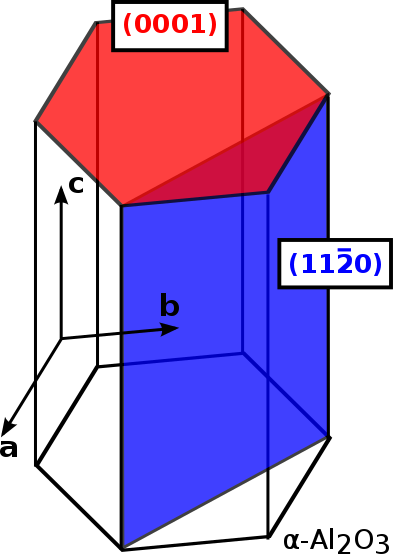
\includegraphics[width=0.30\textwidth]{figures/al2o3-crystal.png}}
             \quad
             %add desired spacing between images, e. g. ~, \quad, \qquad, \hfill etc. (or a blank line to force the subfigure onto a new line)
    \subfigure[(11\=20), top view]{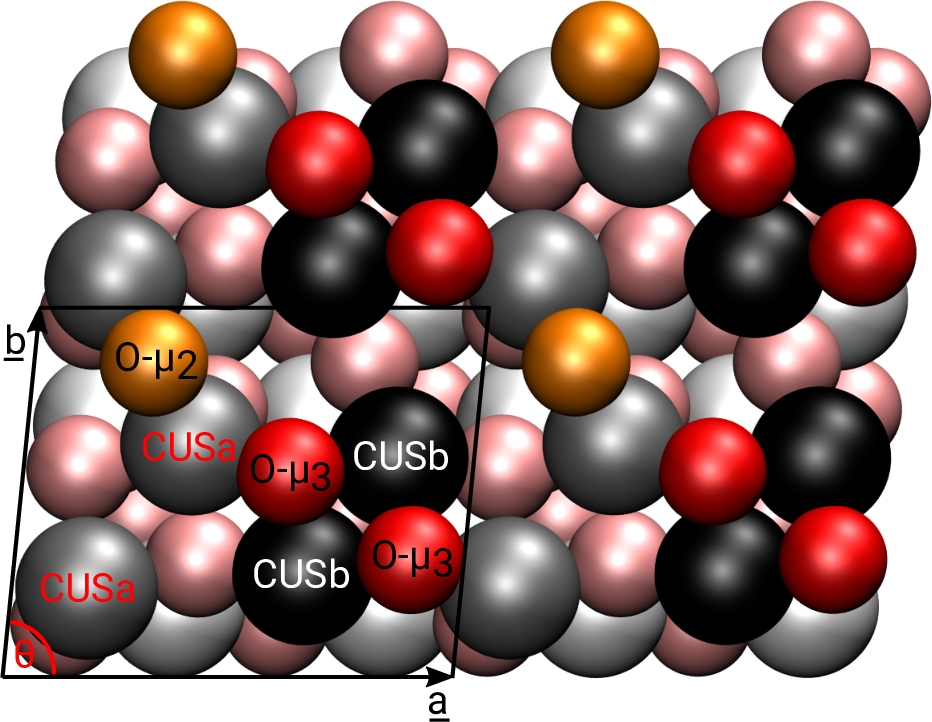
\includegraphics[width=0.30\textwidth]{figures/11-20/supercell_opt.png}}
             \quad
             %add desired spacing between images, e. g. ~, \quad, \qquad, \hfill etc. (or a blank line to force the subfigure onto a new line)
    \subfigure[(11\=20), side view]{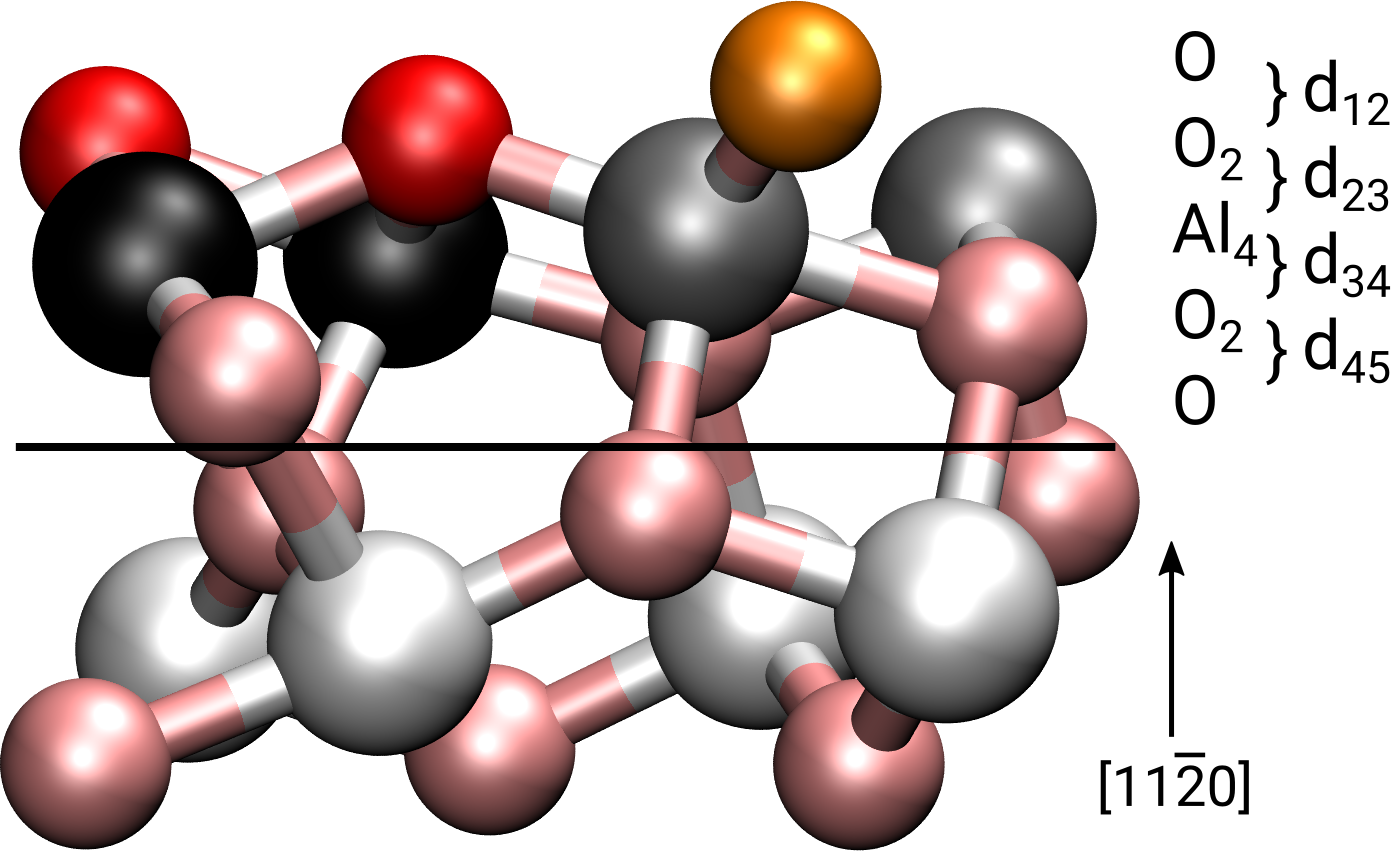
\includegraphics[width=0.30\textwidth]{figures/11-20/uc_opt.png}}
             \caption{.}
            \label{abb:crystal_11-20}
     \end{figure}
\section{Structure Search}
First a low coverage regime was investigated: 1 water molecule per $2\times 2$ supercell, which equals a coverage of 1/12. It was put on different positions on the surface and let relax. We found 1 molecular minimum and several dissociated species including both CUS and oxygen types.
There is also one metastable molecular species that seems more stable than the found molecular minimum, but since there is one imaginary mode displaying the movement of the proton towards the dissociated species this cannot be classified as a stable minimum.
The molecular minimum is substantially less stable than the dissociated species. On the contrary, the dissociated water is very stable, also in comparison with the more stable surface cuts (0001) and (1\=102) that were investigated before in our group.
The dissociated species in direct neighborhood are more stable than those where the proton and the OH residue are further apart, for example because of further diffusion reactions.
Dissociation where the proton is located at a two-fold coordinated surface oxygen is far more stable than the corresponding systems where the three-fold coordinated is occupied.
\\
Also systems with a higher water coverage were considered, tests for 2 water molecules, 4 inter-CUSa$\parallel$O-$\mu_2$ and a fully covered supercell, for these systems also normal mode analyses were done to get IR spectra. 
\begin{figure}[!ht]
 \centering
\subfigure[CUSb]{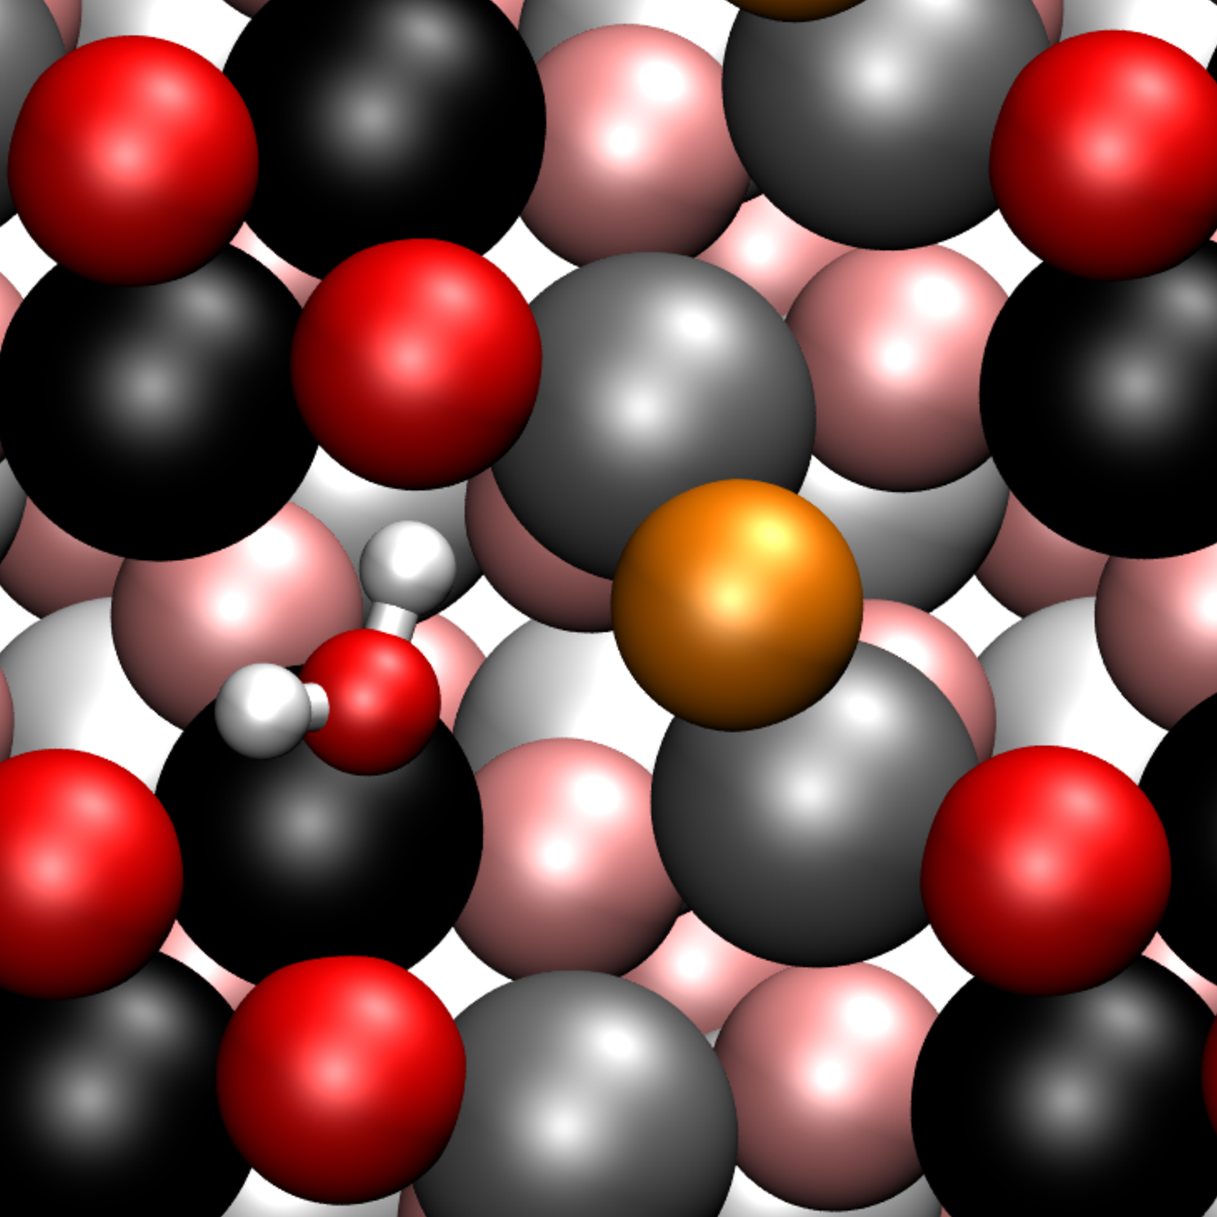
\includegraphics[width=0.2\textwidth]{figures/11-20/test-Cb.pdf}}
 \quad\quad
 \subfigure[inter-CUSa||O-$\mu_2$]{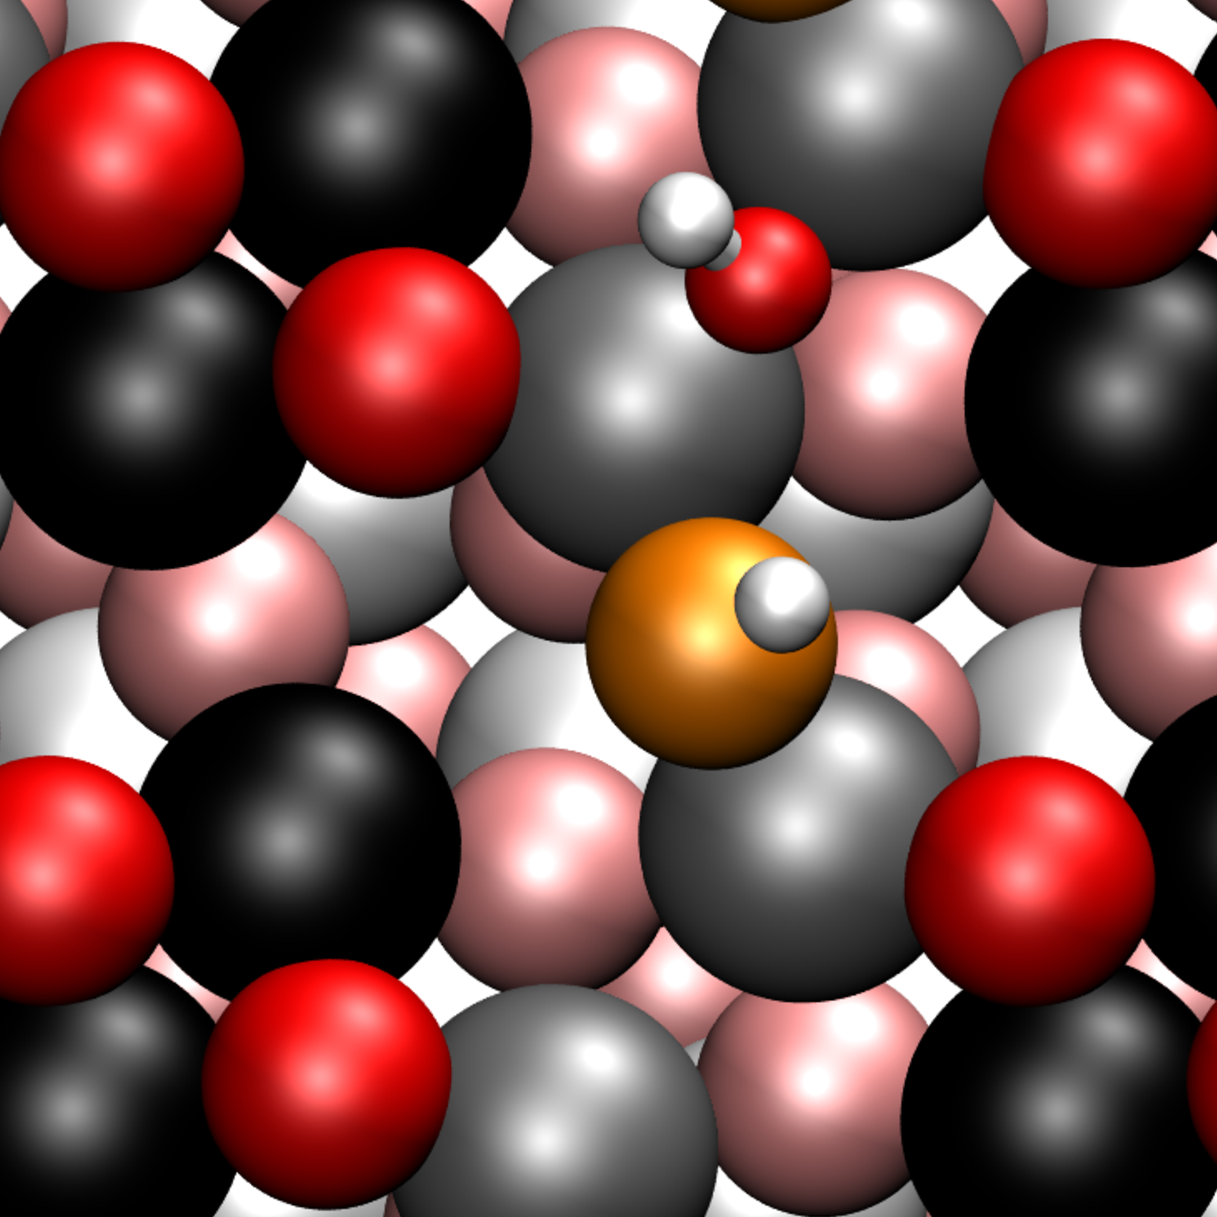
\includegraphics[width=0.2\textwidth]{figures/11-20/test-iCa2.pdf}}
  \quad
\subfigure[CUSb||O-$\mu_2$]{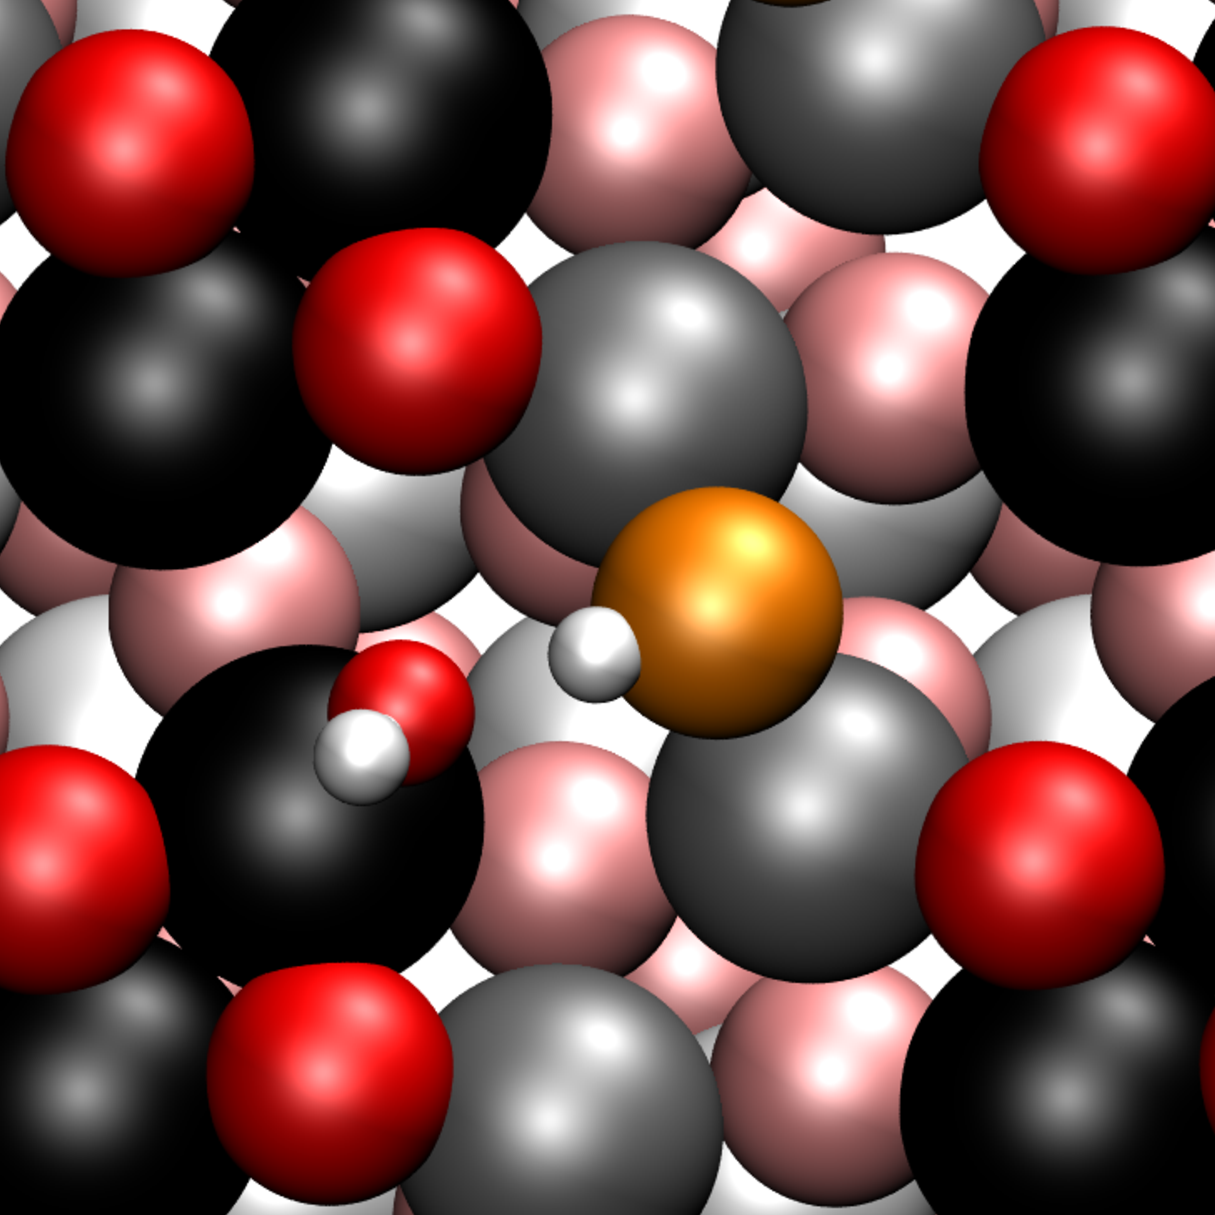
\includegraphics[width=0.2\textwidth]{figures/11-20/test-Cb2.pdf}}
 \quad
\subfigure[inter-CUSb||O-$\mu_2$]{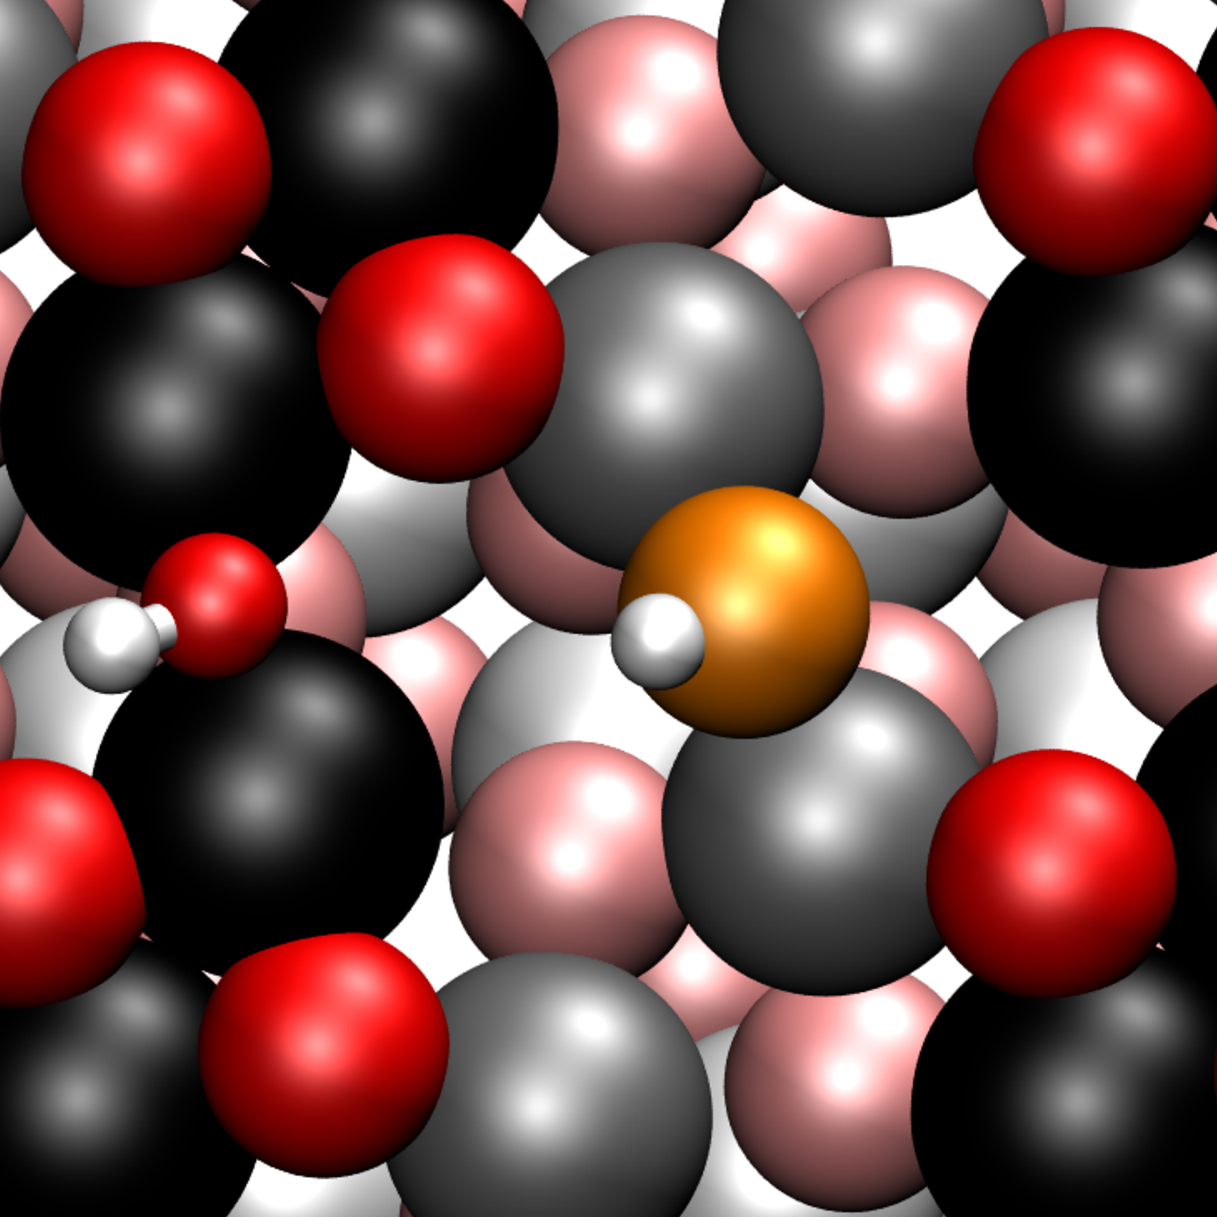
\includegraphics[width=0.2\textwidth]{figures/11-20/test-iCb2.pdf}}
\quad
\subfigure[inter-CUSa||O-$\mu_3$]{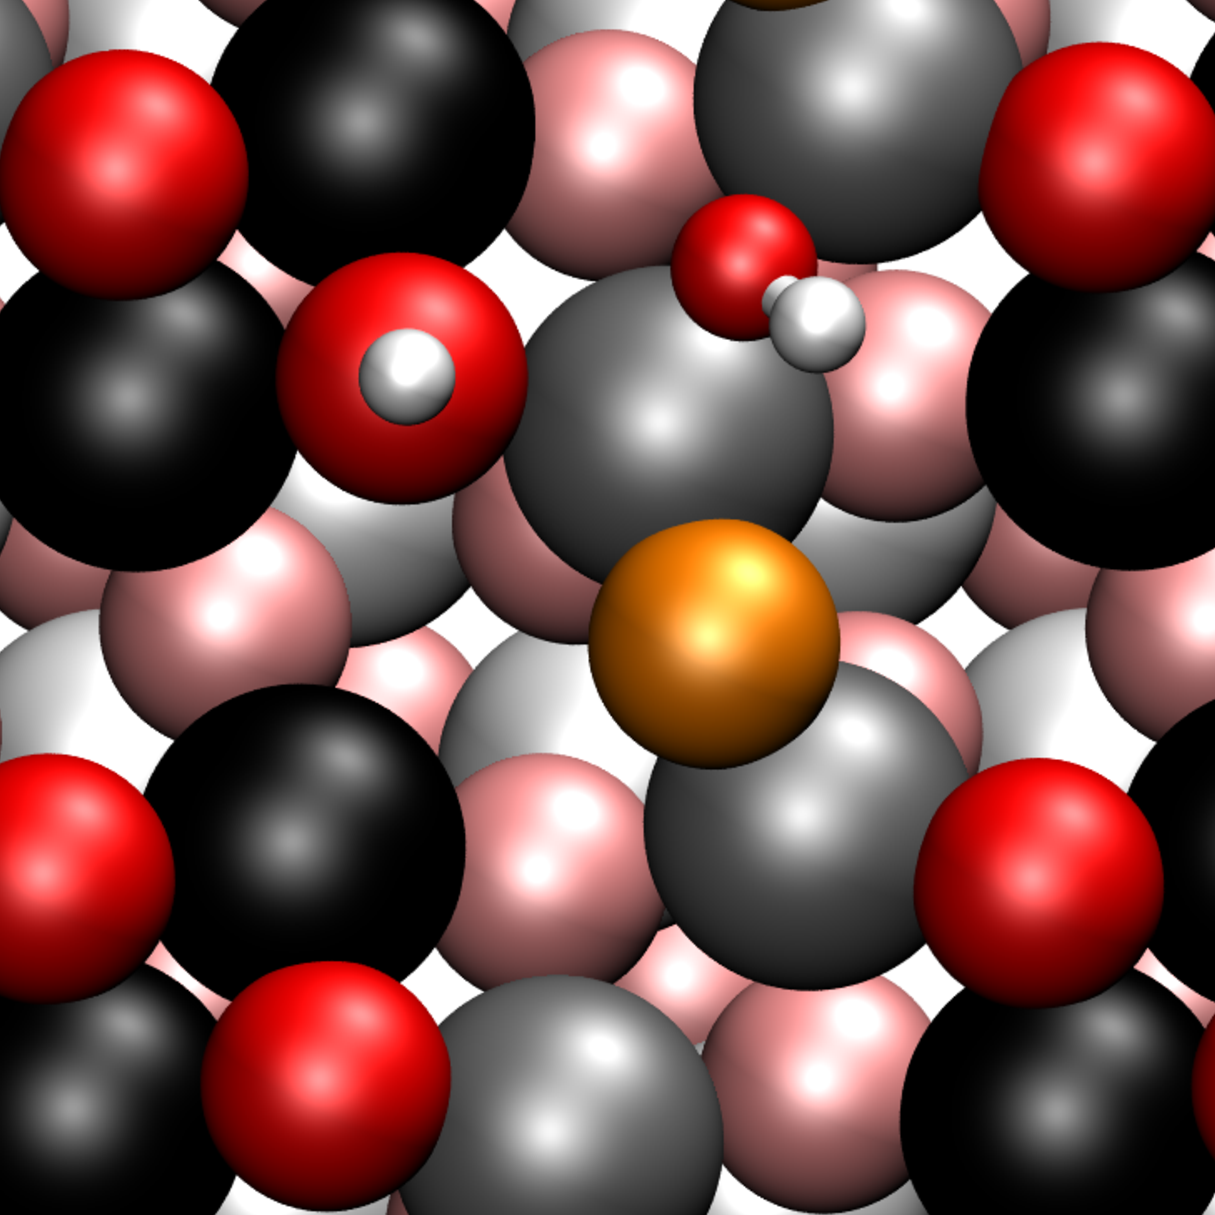
\includegraphics[width=0.2\textwidth]{figures/11-20/test-iCa3.pdf}}
 \quad
\subfigure[CUSb||O-$\mu_3$]{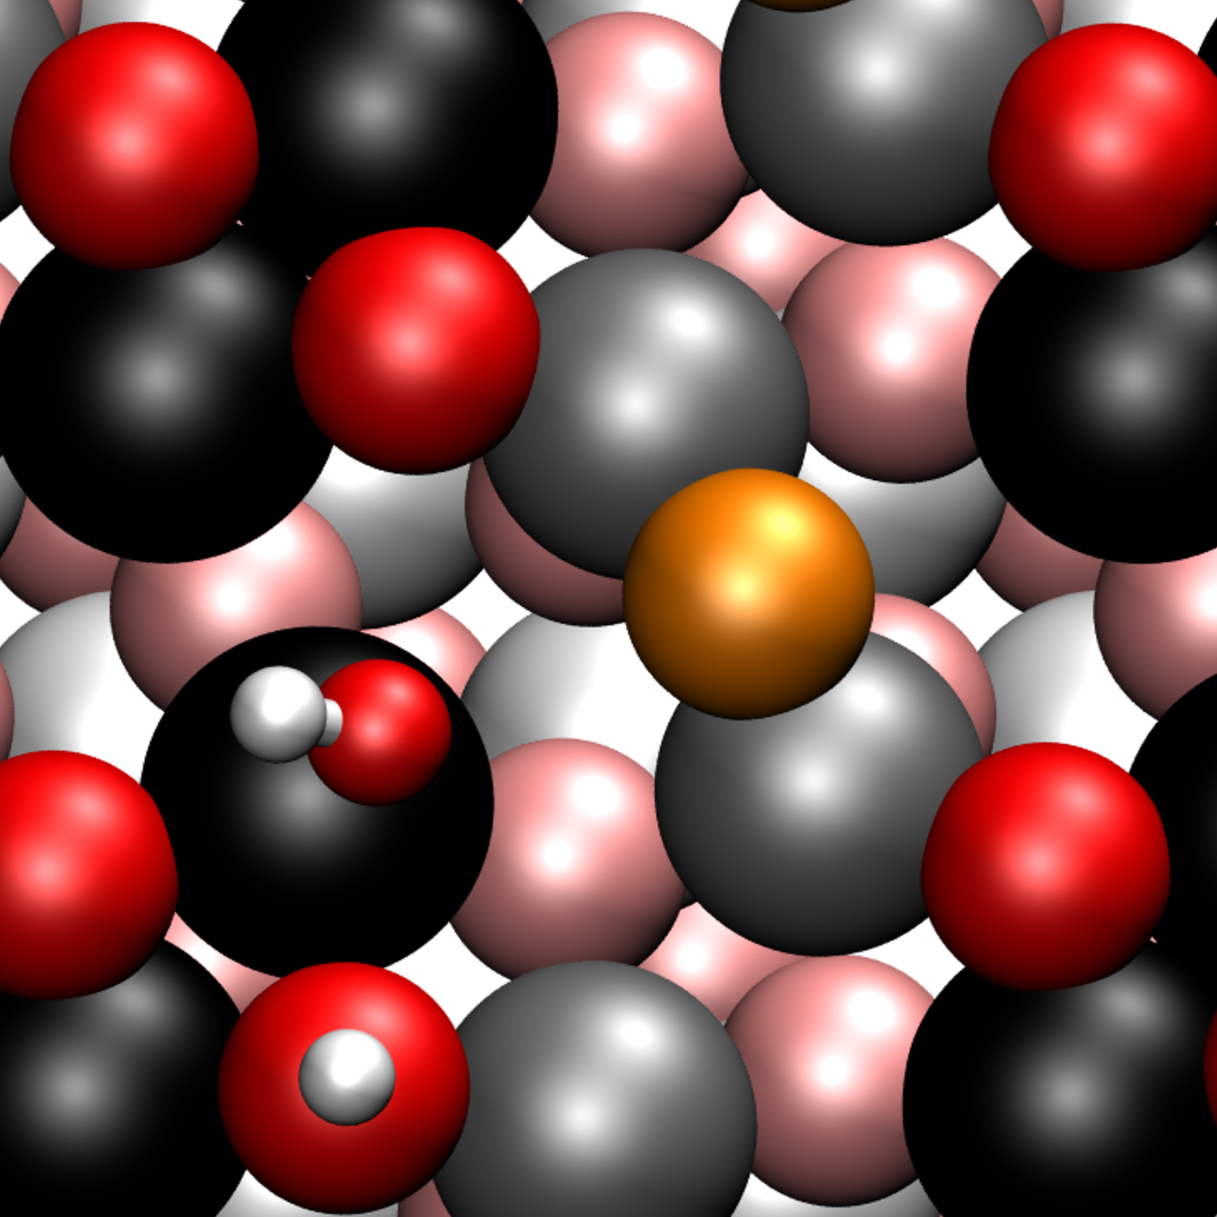
\includegraphics[width=0.2\textwidth]{figures/11-20/test-Cb3.pdf}}
 \quad
\subfigure[inter-CUSb||O-$\mu_3$]{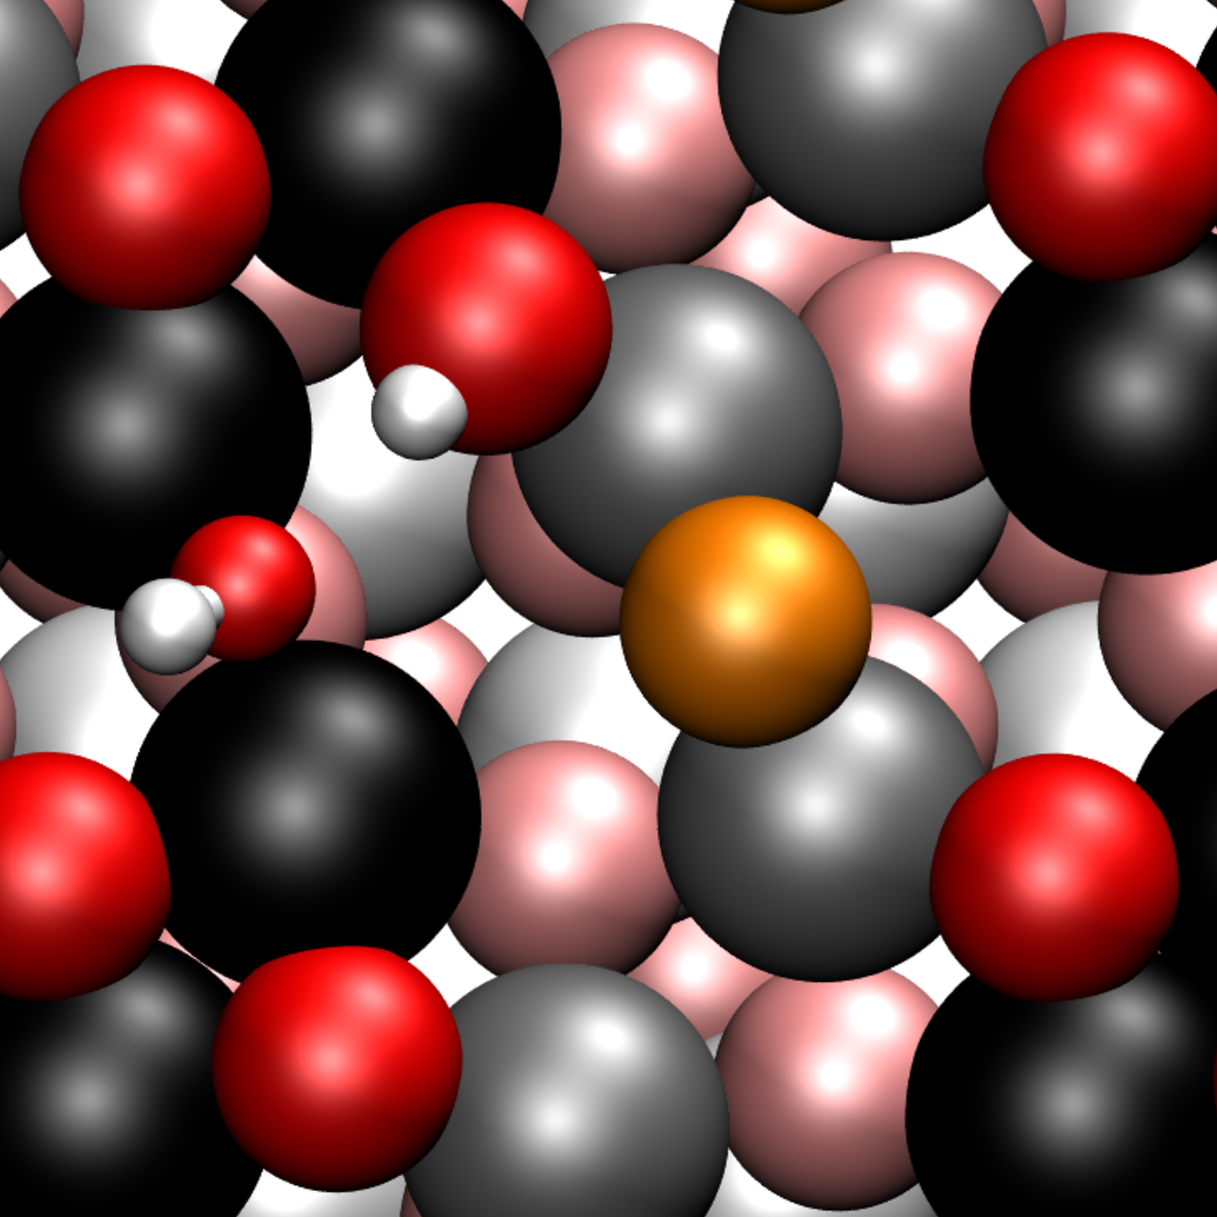
\includegraphics[width=0.2\textwidth]{figures/11-20/test-iCb3.pdf}}
 \caption{{\it change text! Adsorption geometries for molecular (a) and (six) dissociated water 
molecules ((b)-(g)) are shown, as obtained by periodic PBE+D2. The most favorable 
molecularly and dissociatively adsorbed configurations are shown. This means that 
we show nearest neighbor structures only (see text). The color code is the same 
as in Figure \ref{abb:crystal_11-20}(b) and (c), CUSa grey, CUSb black, O-$\mu_2$ orange and O-$
\mu_3$ red; Hydrogen is displayed in white, subsurface layers are in pale colors.}}
        \label{abb:ads-geoms}
 \end{figure}
\section{Frequencies of OH/OD species}
Frequencies for OH and also OD were calculated. Our experimental partner from FHI use D$_2$O instead of H$_2$O because the chemical reactivity is the same but the spectroscopic properties are better with their applied Laser system. The experimental SFG spectra for the OD range is shown in fig.~\ref{abb:exp-sfg}.
\begin{figure}[!ht]
 \centering
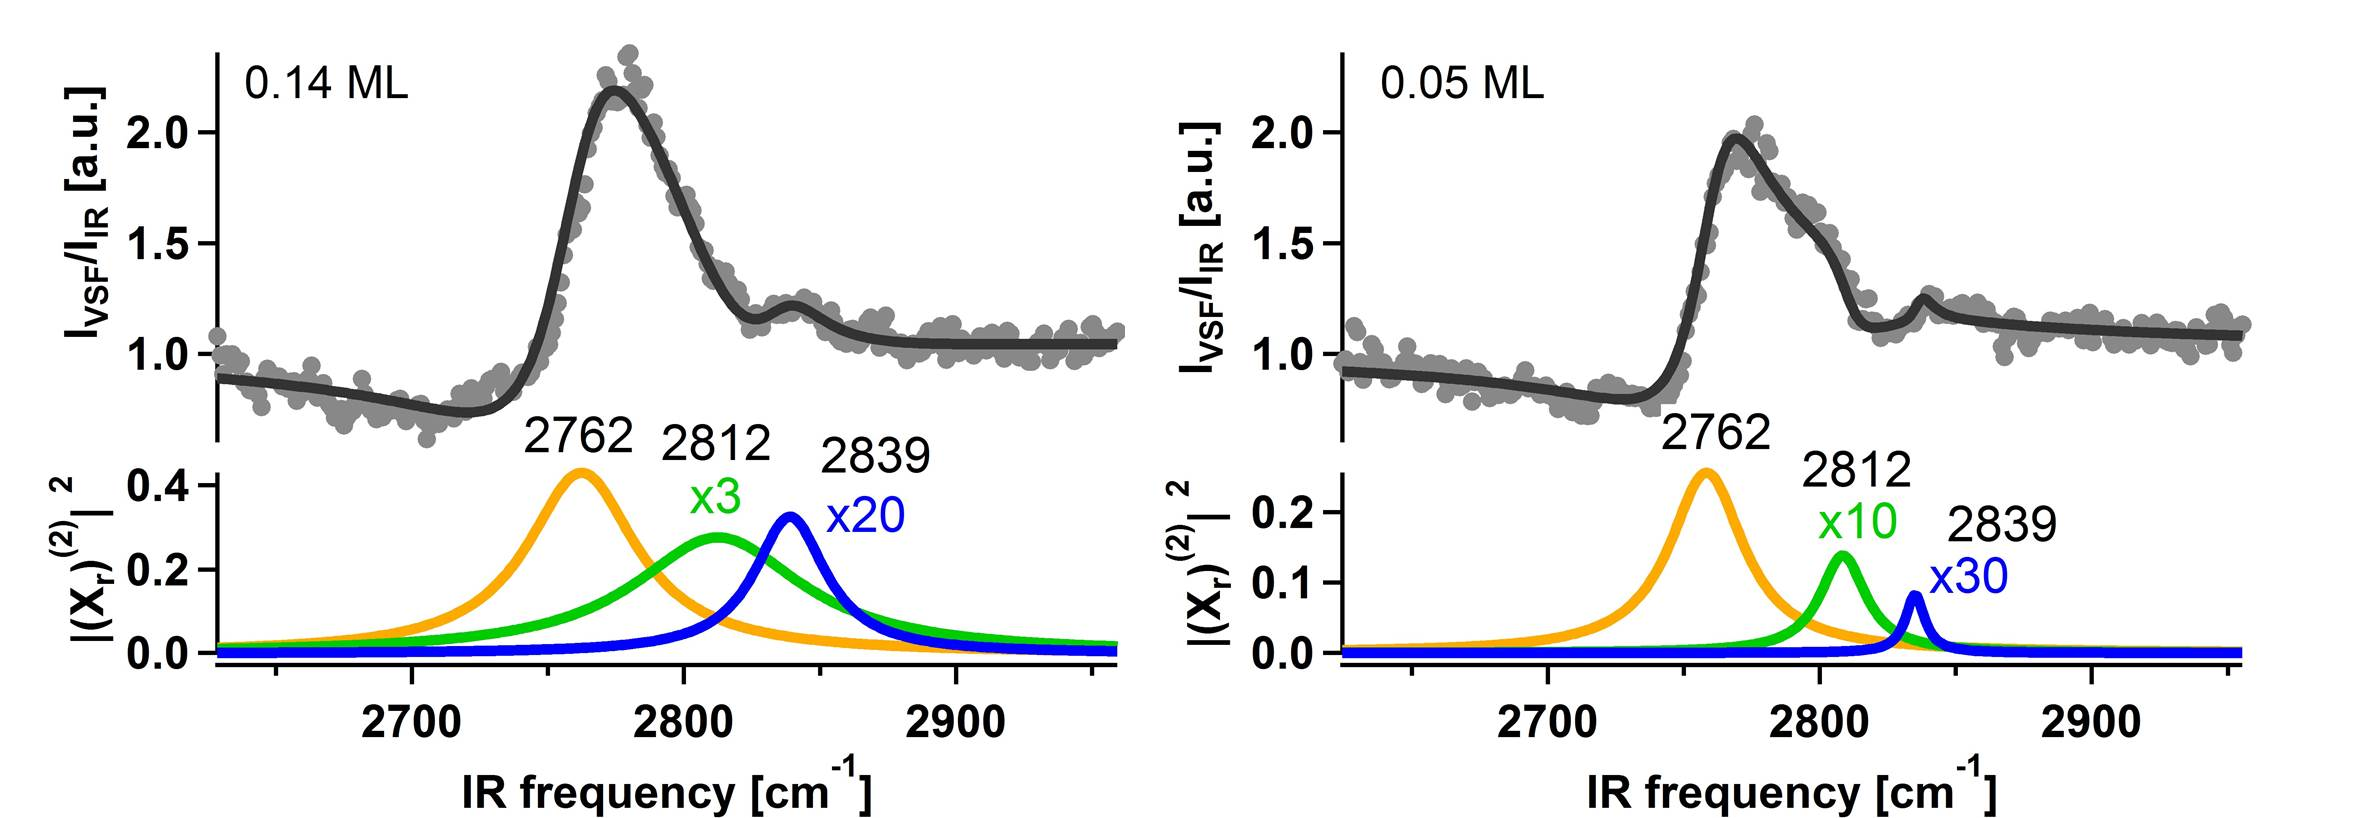
\includegraphics[width=0.9\textwidth]{figures/11-20/SFG_fit.jpg}
 \caption{Experimental SFG results including fit.}
        \label{abb:exp-sfg}
 \end{figure}
Of course, the frequencies for a deuterated system are different from OH, but the isotope can be calculated easily within vasp.
Listed all frequencies for all possible next neighboring structures are shown but in comparison with the experiment, we only focus on the 3 most stable adsorbate structures, since only those are expected to be seen in experiment.
\\
Also results for higher coverage.

\subsection{Normal Mode Analysis}
The classical modes calculated with a normal mode analysis are dependent on the mass and the spring constant of the bond.
We assumed that the OH/OD stretching modes for the 3 most stable structures (of course for all others as well in order to check whether a structure is a minimum) would contribute to the spectrum the most. Following this approach we expect 6 modes (2 for each, one of the adsorbed OH group and one for the surface group). We expect 6 frequencies. when evaluating those values one can see that one is out of the experimental range (strongly hydrogen bonded species, wave number is shifted to low $\tilde{\nu}$ and some of the others are except for numerical differences the same, so there should be only 3 bands visible. Very good agreement with the experimental modes. The numbers itself do not compare too good, but the relative modes are in really good agreement.
\\
Comparison of different slab sizes.
\\
Comparison of intensities with dipole corrections and Born effective charges.

\subsection{Velocity-Velocity Autocorrelation Function}
Extract vel vel autocorrelation function from MD at $300\,$K (and also $400\,$K?) from most stable structures (inter-CUSa||O-$\mu_2$, CUSb||O-$\mu_2$ and inter-CUSb||O-$\mu_2$), with Fourier transformation converted to VDOS spectrum. It also is possible to separate Modes from water layers from bulk phonons. Not really important if you don't use hydroxylated surface with a higher water coverage?

\section{Reactions and Microkinetic Model}
Based on the minimum structures one has to identify reaction pathways to fully understand a system, so we utilize the NEB method including Climbing Image to search for transition states between the minima. We examined 3 types of reactions: dissociation, OH-diffusion and H-diffusion. Since the molecular minimum is very low in stability, and also the barrier is very low for the process. 
Also tried to study the adsorption/desorption process but didn't find a barrier, energy profile behaves smoothly from water molecule above the surface to the adsorbed water system.
\\
Problem of GGA underestimating barriers is well known. {\color{red} Optimizing structure with HSE06 is nearly impossible due to high cost and doing single point calculations on the PBE transition state is not very accurate and doesn't deliver better results. (at least for crystal calculations... so don't bring it her?)}
\\
For the OH diffusion we find  that a special case of CUSb to inter-CUSb diffusion is favored, because the distance that has to be brigded is very small; but real CUS to CUS diffusion like the one from CUSb to inter-CUSa is very slow.
\\
{\color{red} TEST?? What doesn't work is the molecular diffusion from CUSb to CUSb, the molecular minimum is not stable enough, during the path, dissociation would occur? Or it would have to be a two step reaction from CUSb to inter-CUSb what does not exist and then further to CUSb..}
\\
Proton diffusion reactions are way more variable giving reaction rates at $300\,$K ranging from $10^{-x}$ to $10^{+y}$s$^{-1}$. The barriers and therefore also rate constants for H-diffusion cover a wider range depending on the distance between OH and H and of course more importantly on the fact between which type of O$\mu_2$ the proton is diffusing.
\\
Also reactions leading to a not next-neighbored situation, increasing the distance between OH and H are also not favorable since gemoetries with the residues further apart are energetically less stable.

\begin{figure*} [!ht]
\centering
\subfigure[D-I: CUSb $\rightarrow$CUSb||O-$\mu_2$]{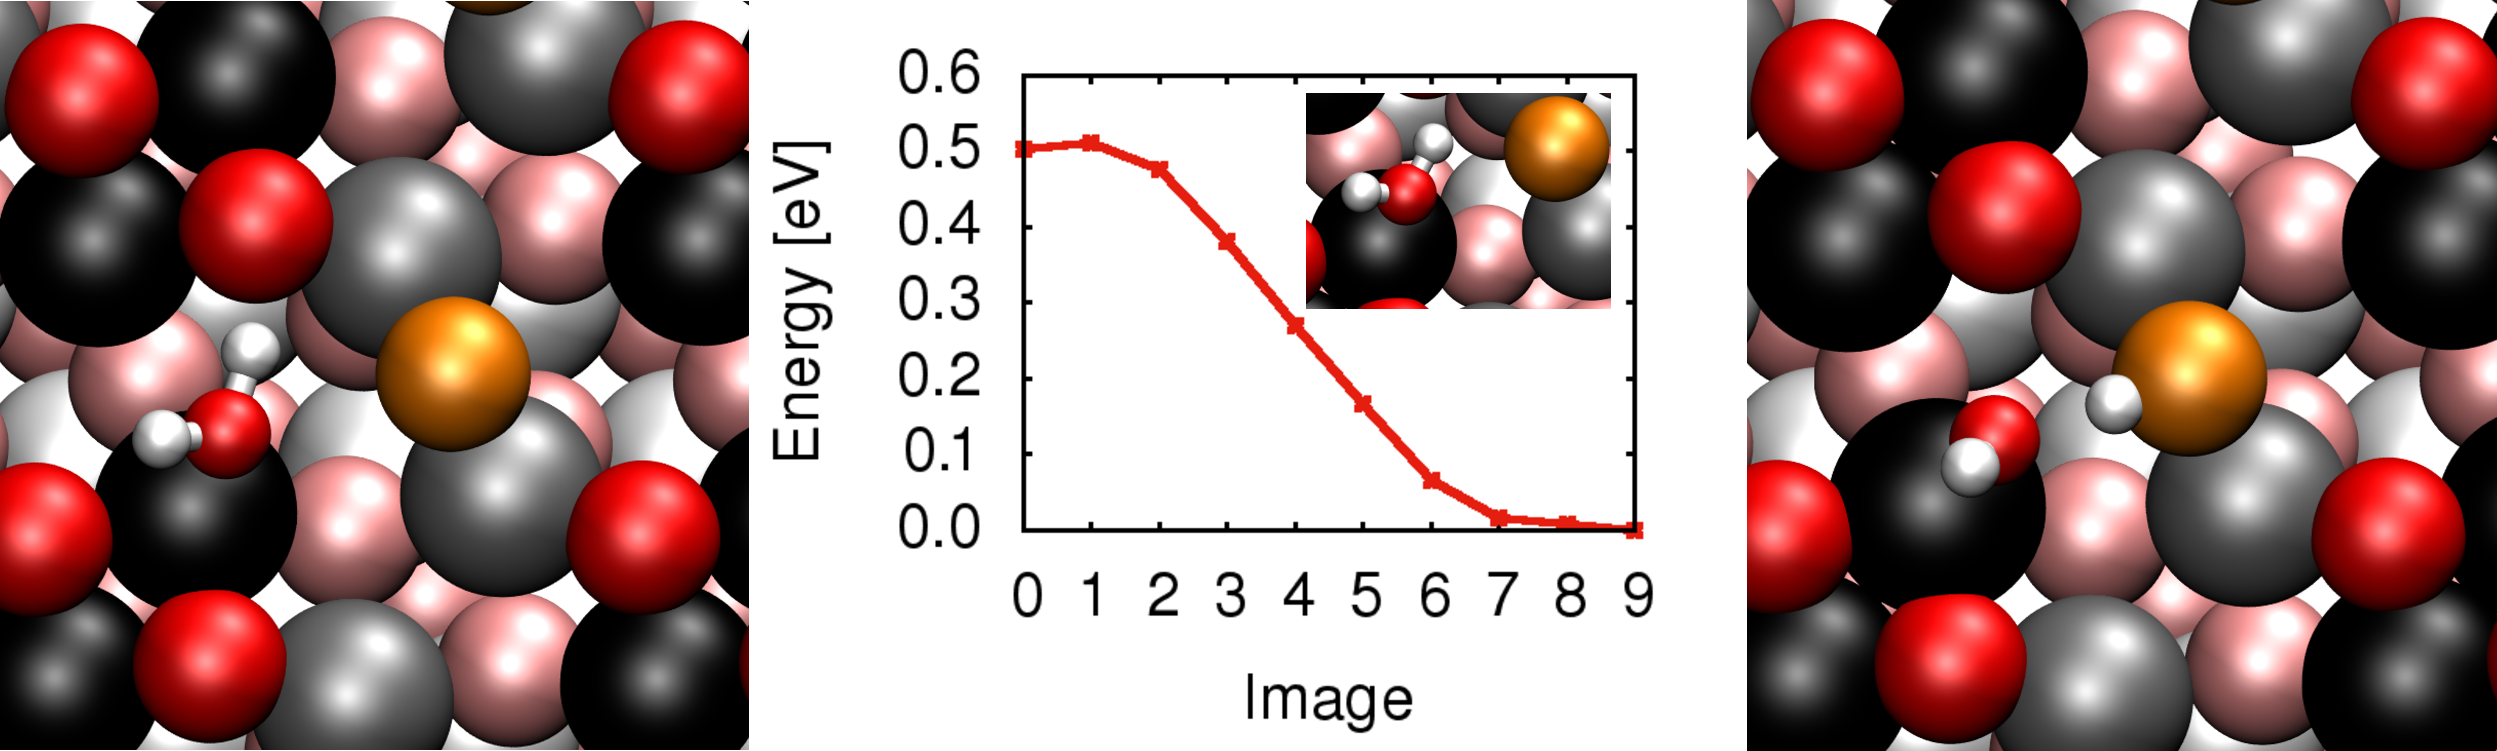
\includegraphics[width=0.7\textwidth]{figures/11-20/Diss_Cb-Cb2.pdf}}
         \quad
\subfigure[D-II: CUSb $\rightarrow$CUSb||O-$\mu_3$]{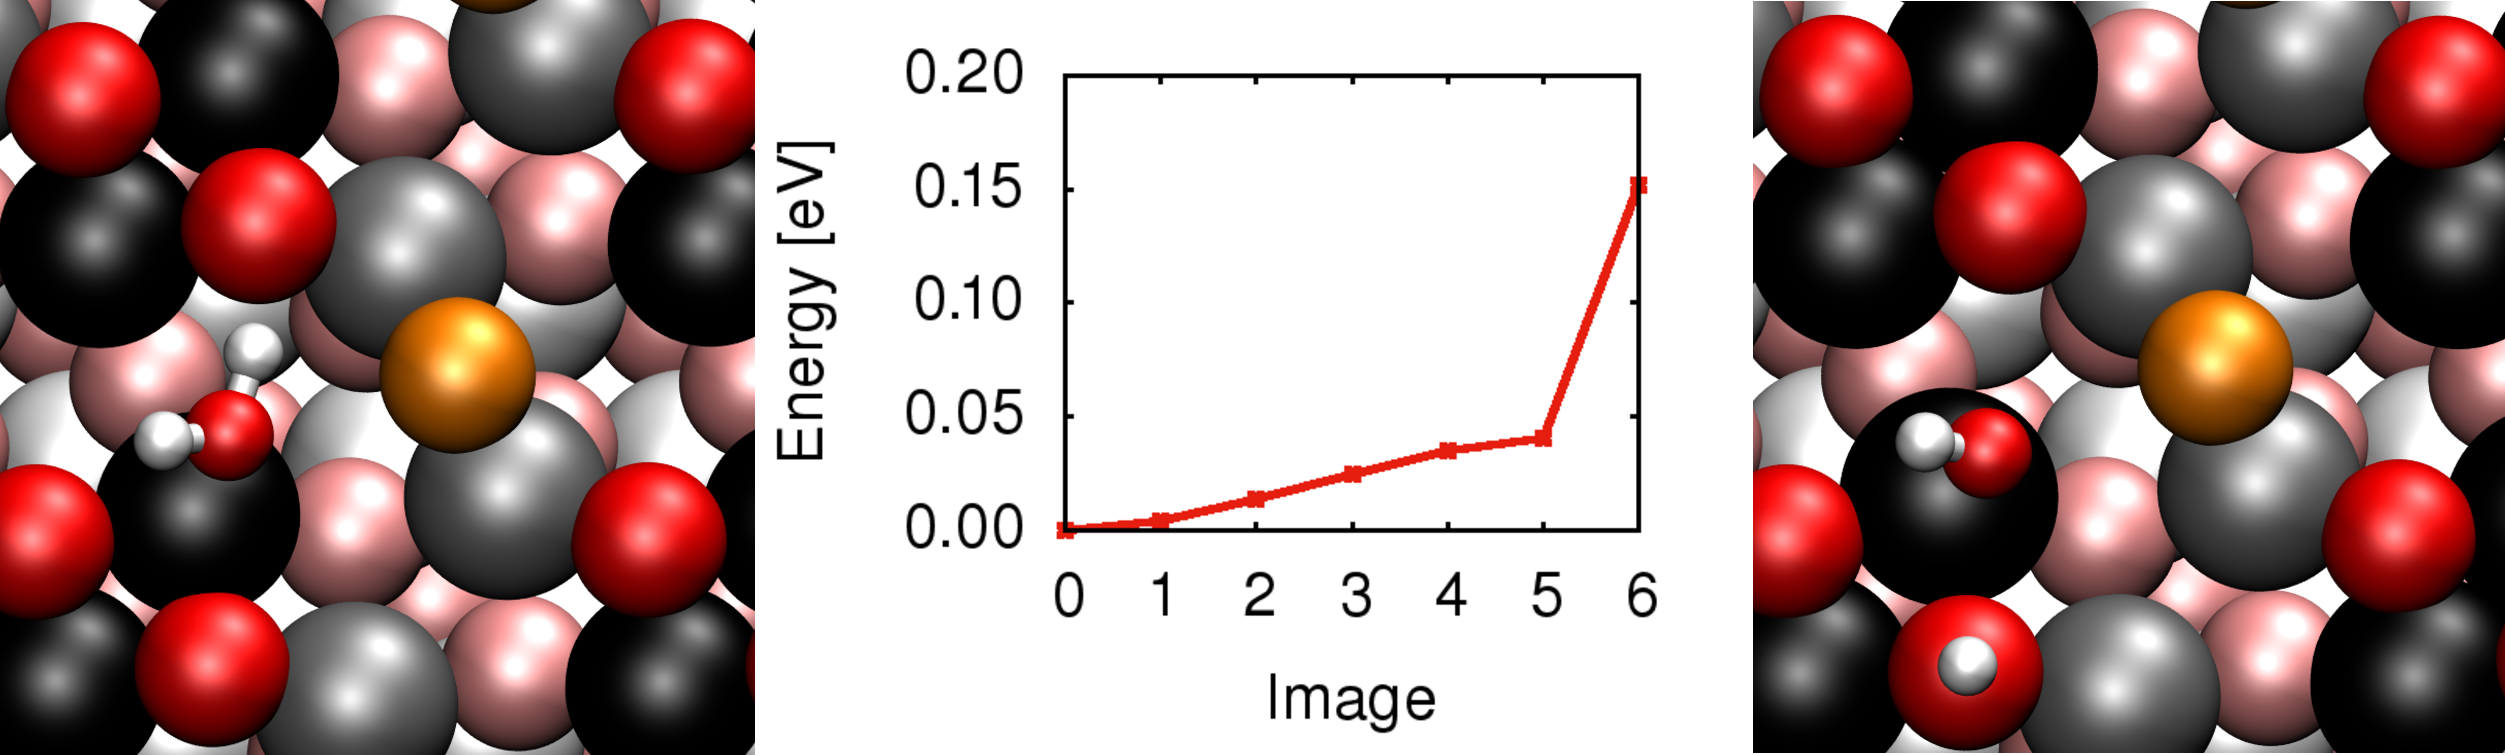
\includegraphics[width=.7\textwidth]{figures/11-20/Diss_Cb-Cb3.pdf}}
 \quad
\subfigure[Df-OH-III: CUSb||O-$\mu_2$ $\rightarrow$inter-CUSb||O-$\mu_2$]{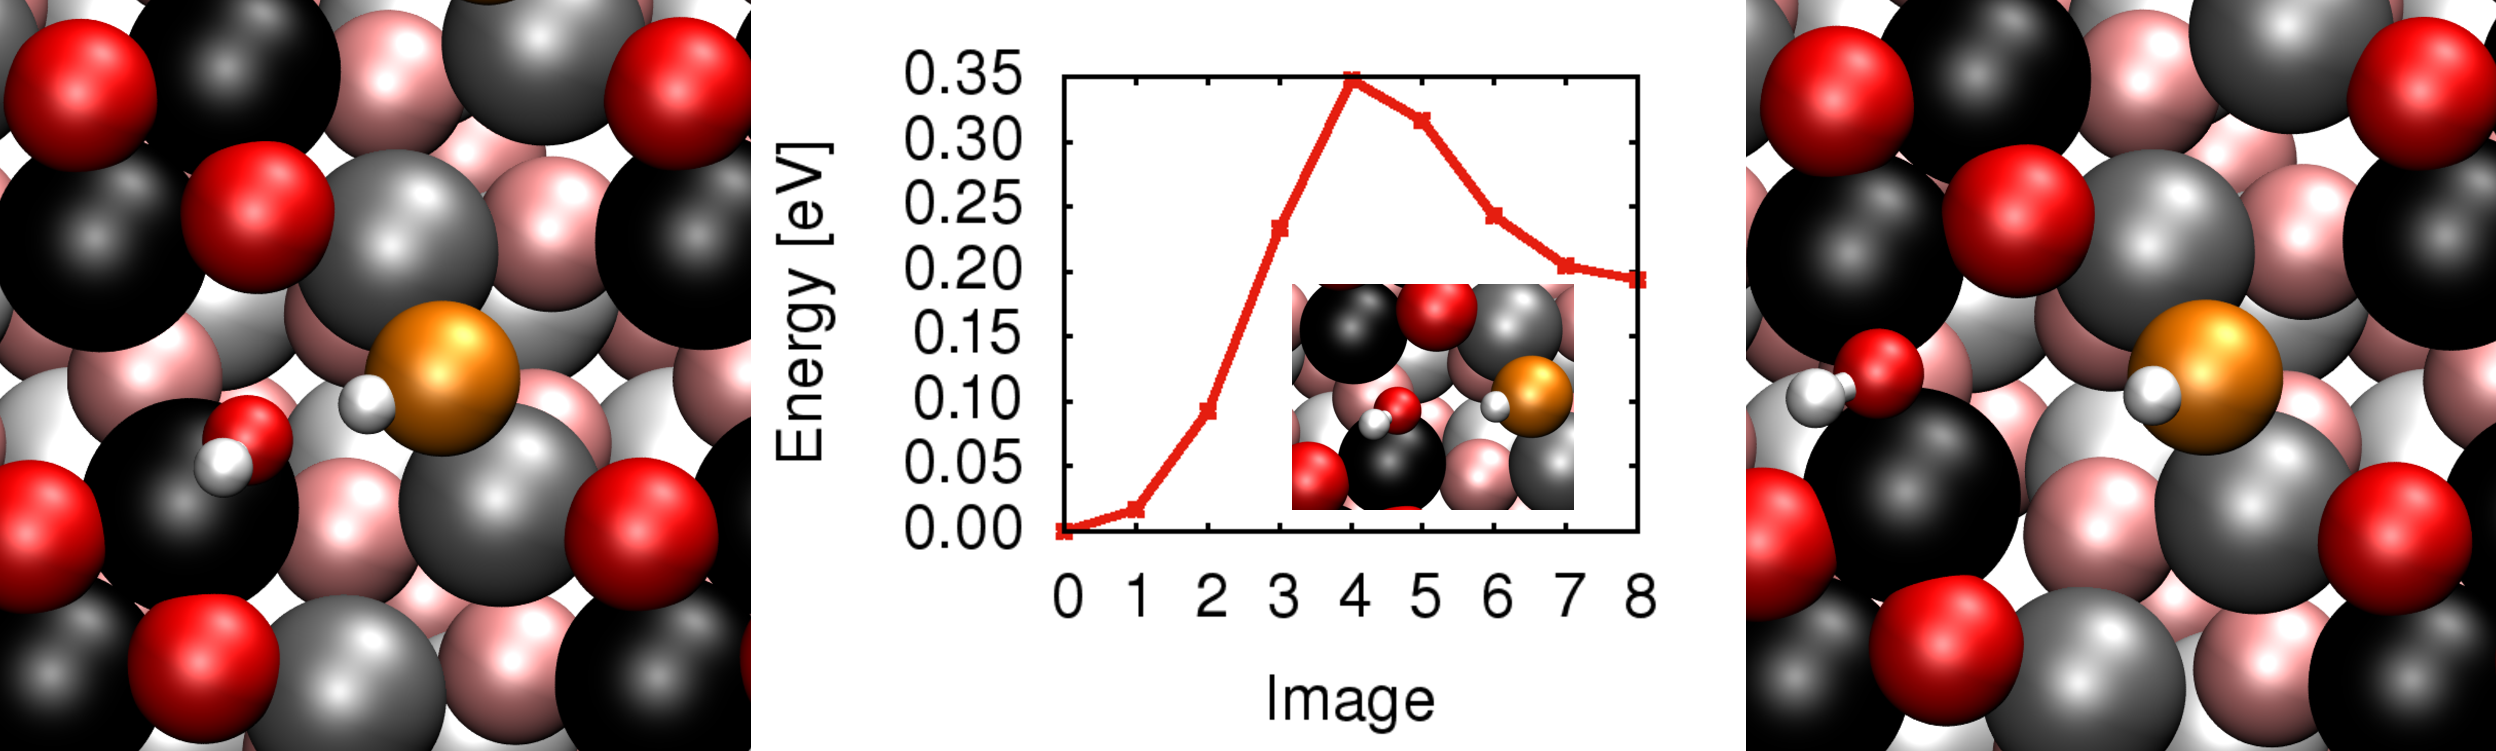
\includegraphics[width=.7\textwidth]{figures/11-20/Diff-OH_Cb2-iCb2.pdf}}
 \quad
\subfigure[Df-OH-IV: CUSb||O-$\mu_2$ $\rightarrow$inter-CUSa||O-$\mu_2$]{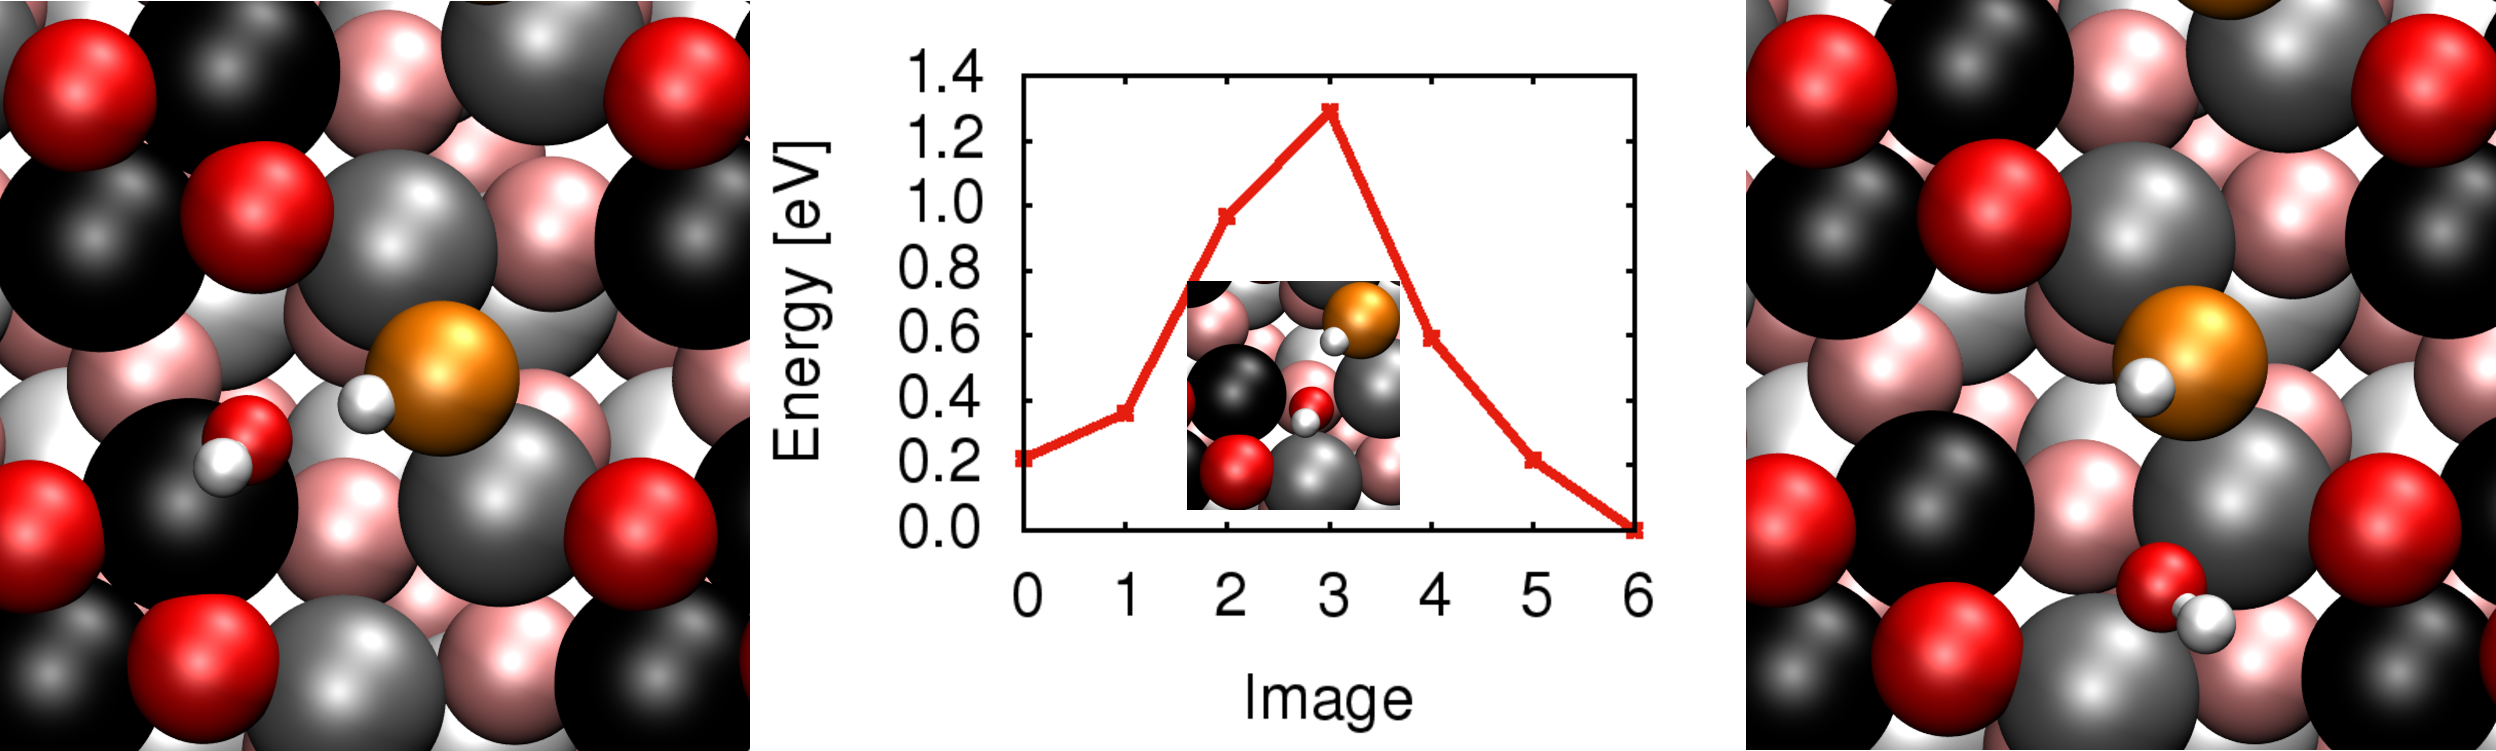
\includegraphics[width=.7\textwidth]{figures/11-20/Diff-OH_Cb2-iCa2.pdf}}
\caption{PBE+D2 minimum energy paths with transition states (inlay; if available), 
  and both educt (left) and product (right) states for D-I, D-II, Df-OH-III and Df-OH-IV reactions, respectively. The color code is as explained above.}
       \label{mep}
\end{figure*}
\begin{figure*} [!ht]
\centering
\subfigure[Df-H-V: inter-CUSa||O-$\mu_2\rightarrow$inter-CUSa||O-$\mu_3^\prime$]{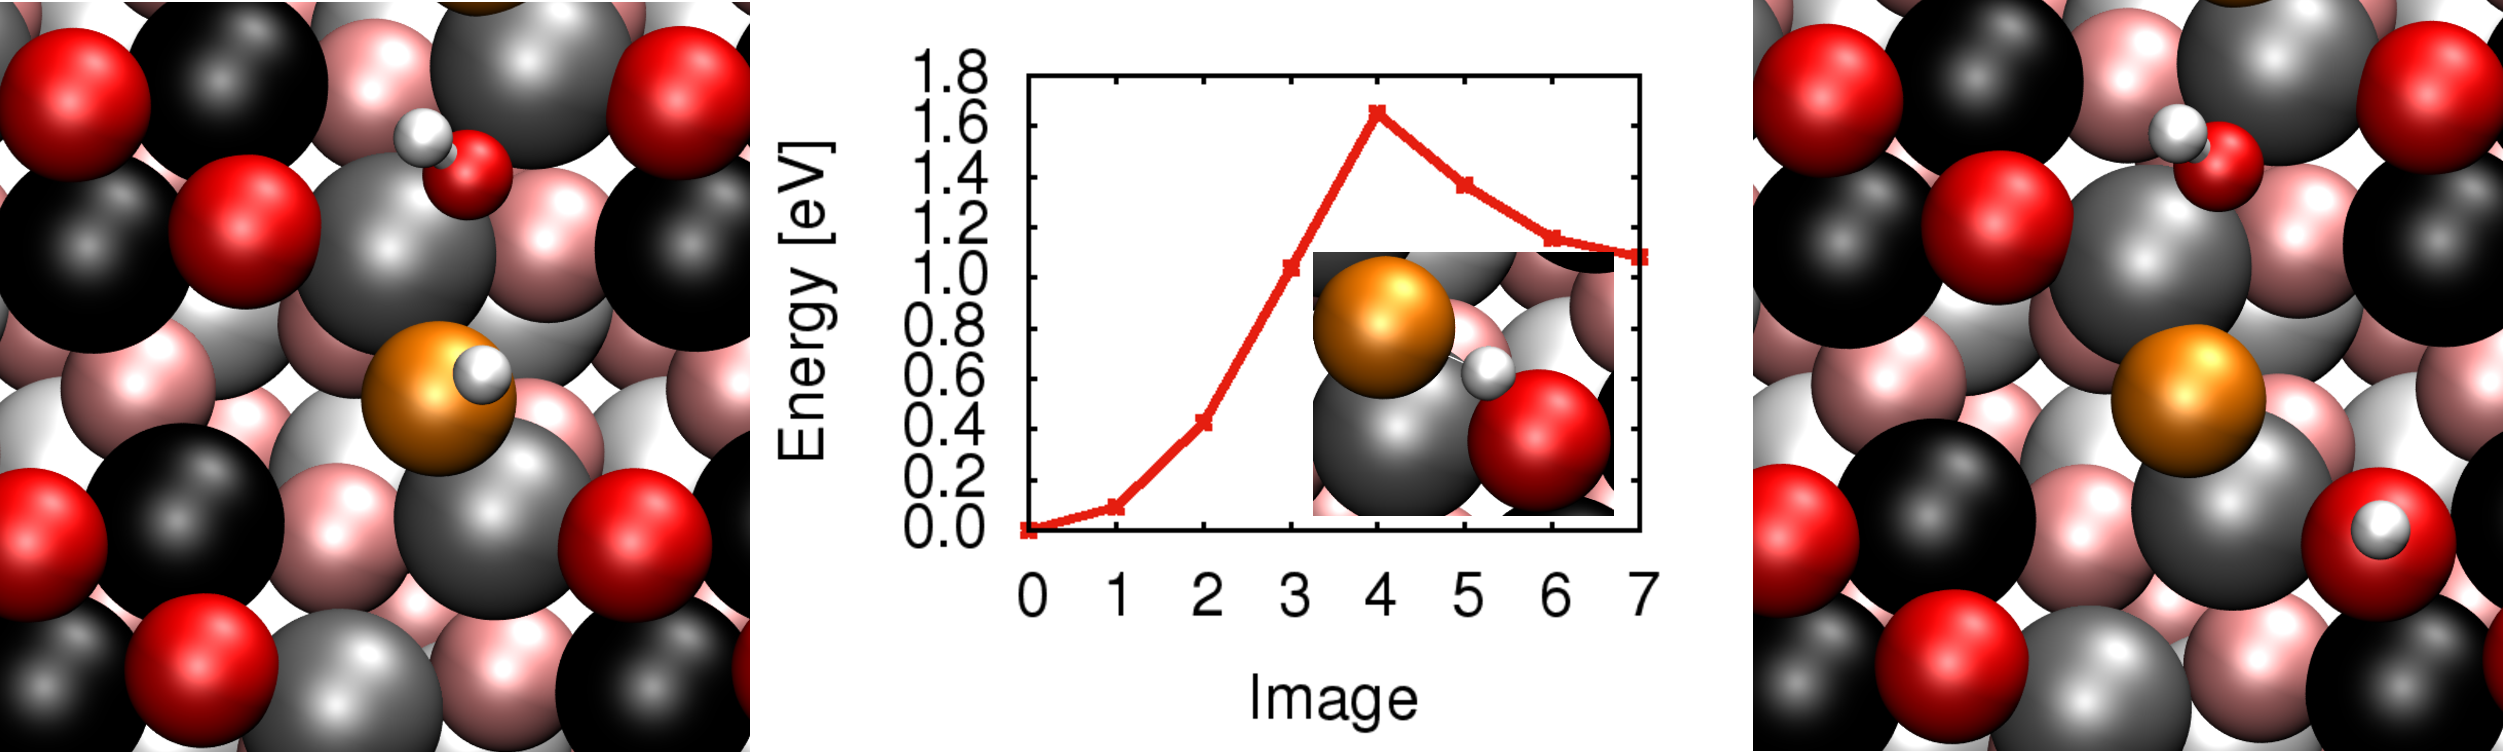
\includegraphics[width=.7\textwidth]{figures/11-20/Diff-H_iCa2-iCa3p.pdf}}
 \quad
\subfigure[Df-H-VI: inter-CUSb||O-$\mu_3^{\prime\prime}$ $\rightarrow$inter-CUSb||O-$\mu_3^{\prime\prime\prime}$]{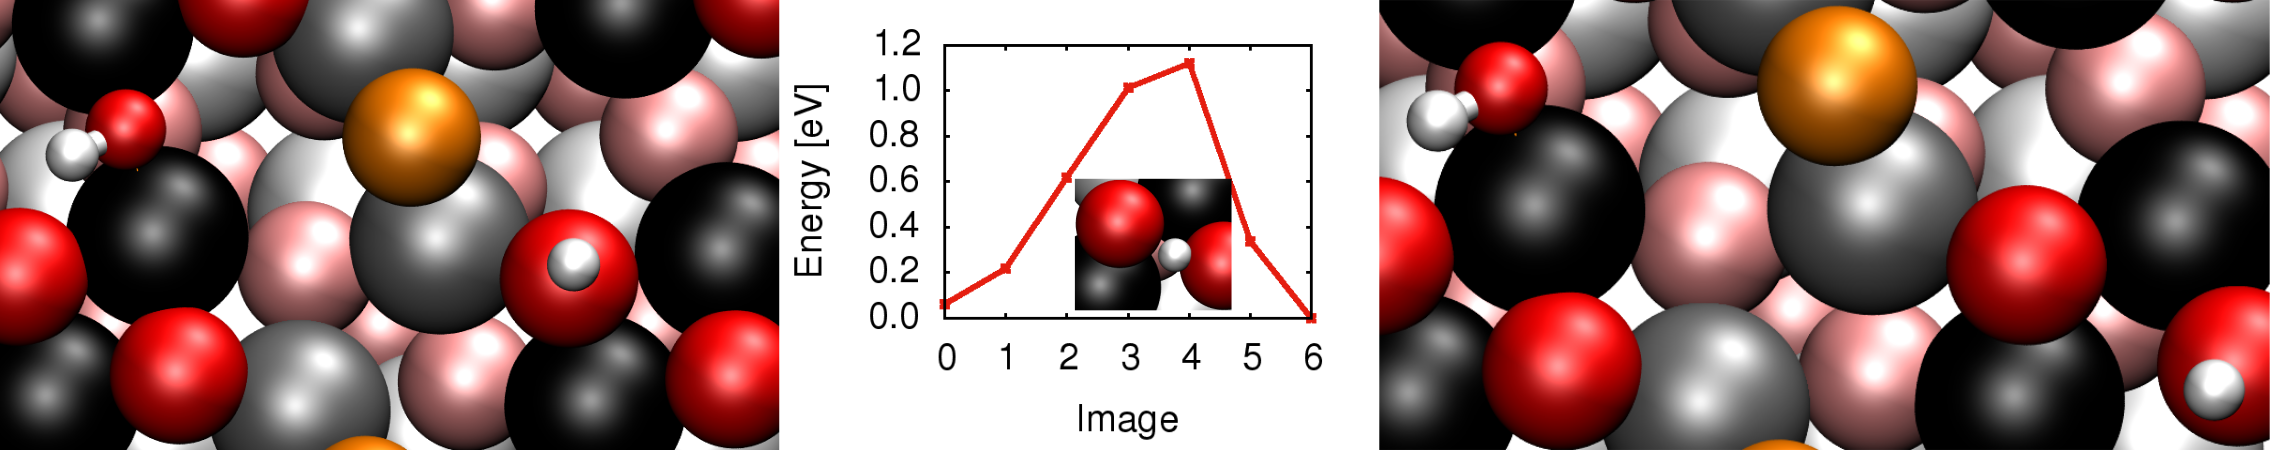
\includegraphics[width=.7\textwidth]{figures/11-20/Diff-H_iCb3pp-iCb3ppp.png}}
\caption{PBE+D2 minimum energy paths with transition states, and both educt and product states for Df-H-V and Df-H-VI reactions, respectively. The color code is as explained above.}
       \label{mep2}
\end{figure*}

\section{Phonons}
For the phonons as a first test the same normal modes analyses were checked to get a first impression into how the spectra can look like. But for a better description we need to consider more layers of the bulk in order to get more reliable results. From an experimental point of view it is suggested that SFG spectra can give insight into {\color{red} x} layers of the bulk. Therefore we did calculations for the most stable adsorption geometries for more layered systems, going up to 6*5=30 layers, both for the naked surface and for the covered surface, here we used again optimized geometries of the most stable structures. These results are also shown with intensities calculated from dipole corrected normal mode analyses.

\section{Desorption Process}
As mentioned before the experimentalists measure TPD in order to understand the adsorption strength and possible exchange reactions. We tried to simulate the desorption process using the following scheme: take the water in the gas phase + the naked surface as the standard. In the thermal equilibrium, the water should be equally distributed to Boltzman's distribution in the most stable structures. From this situation the water can recombine to the molecularly adsorbed water. The recombined water then can desorb to the gas phase. Since the spectrum is measured in ultra high vacuum it can be assumed that all the water that has left the surface will not return to the system, because it is dragged out of the equilibrium by the vacuum pumps.
Applying the reaction rates of the corresponding reactions in a kinetic Monte Carlo approach leads to 
{\color{red} REDO THESE CALCULATIONS}.

\chapter{Water on $\upalpha$-Al$_2$O$_3$(0001)}
The most stable surface site under UHV conditions, subject of several studies so far.
\section{Surface Model}
Crystal structure of $\upalpha$-Al$_2$O$_3$ with surface cuts (0001) and (11\=20) in comparison.
We applied here a $2\times 2$ supercell with, as before, vectors as in the bulk (did Jonas optimize them?) Al terminated surface, only one type of CUS, all oxygen atoms are 3-fold coordinated, topography is not as complicated as for the higher indexed surface. x layers, y fixed.
\\
1 Water  molecule per $2\times 2$ supercell was already studied by Dr. Jonas Wirth, but in order to understanf the chemistry, one has to know how water reacts in this system. There is one molecular minimum on top of a CUS atom and mainly 3 dissociated states, the next neighboring 1-2 dissociated state, the 1-4 dissociated structure with the Hydrogen atom being one position further and the 1-4$^\prime$ that is the configuration with the greatest distance that is possible for this slab size. The 1-2 diss is the most stable on and the 1-4$^\prime$ is the least stable one. For the molecular and the 1-4 diss, the stability is, depending on the method, but lies between the previously mentioned ones, for some methods PW91+D2(?) it is the same adsorption energy (the value is calculated as for the (11\=20)), or for some methods and basis sets tested with crystal the one or the other is more stable.
\\
Of course there are reactions linking these minima, dissociation, OH- and H-diffusion were studied, as well as rotation of a OH group and molecular water diffusion from CUS to CUS. The latter two do not play a crucial role in this work.
\begin{figure}[!ht]
 \centering
\subfigure[(0001), top view]{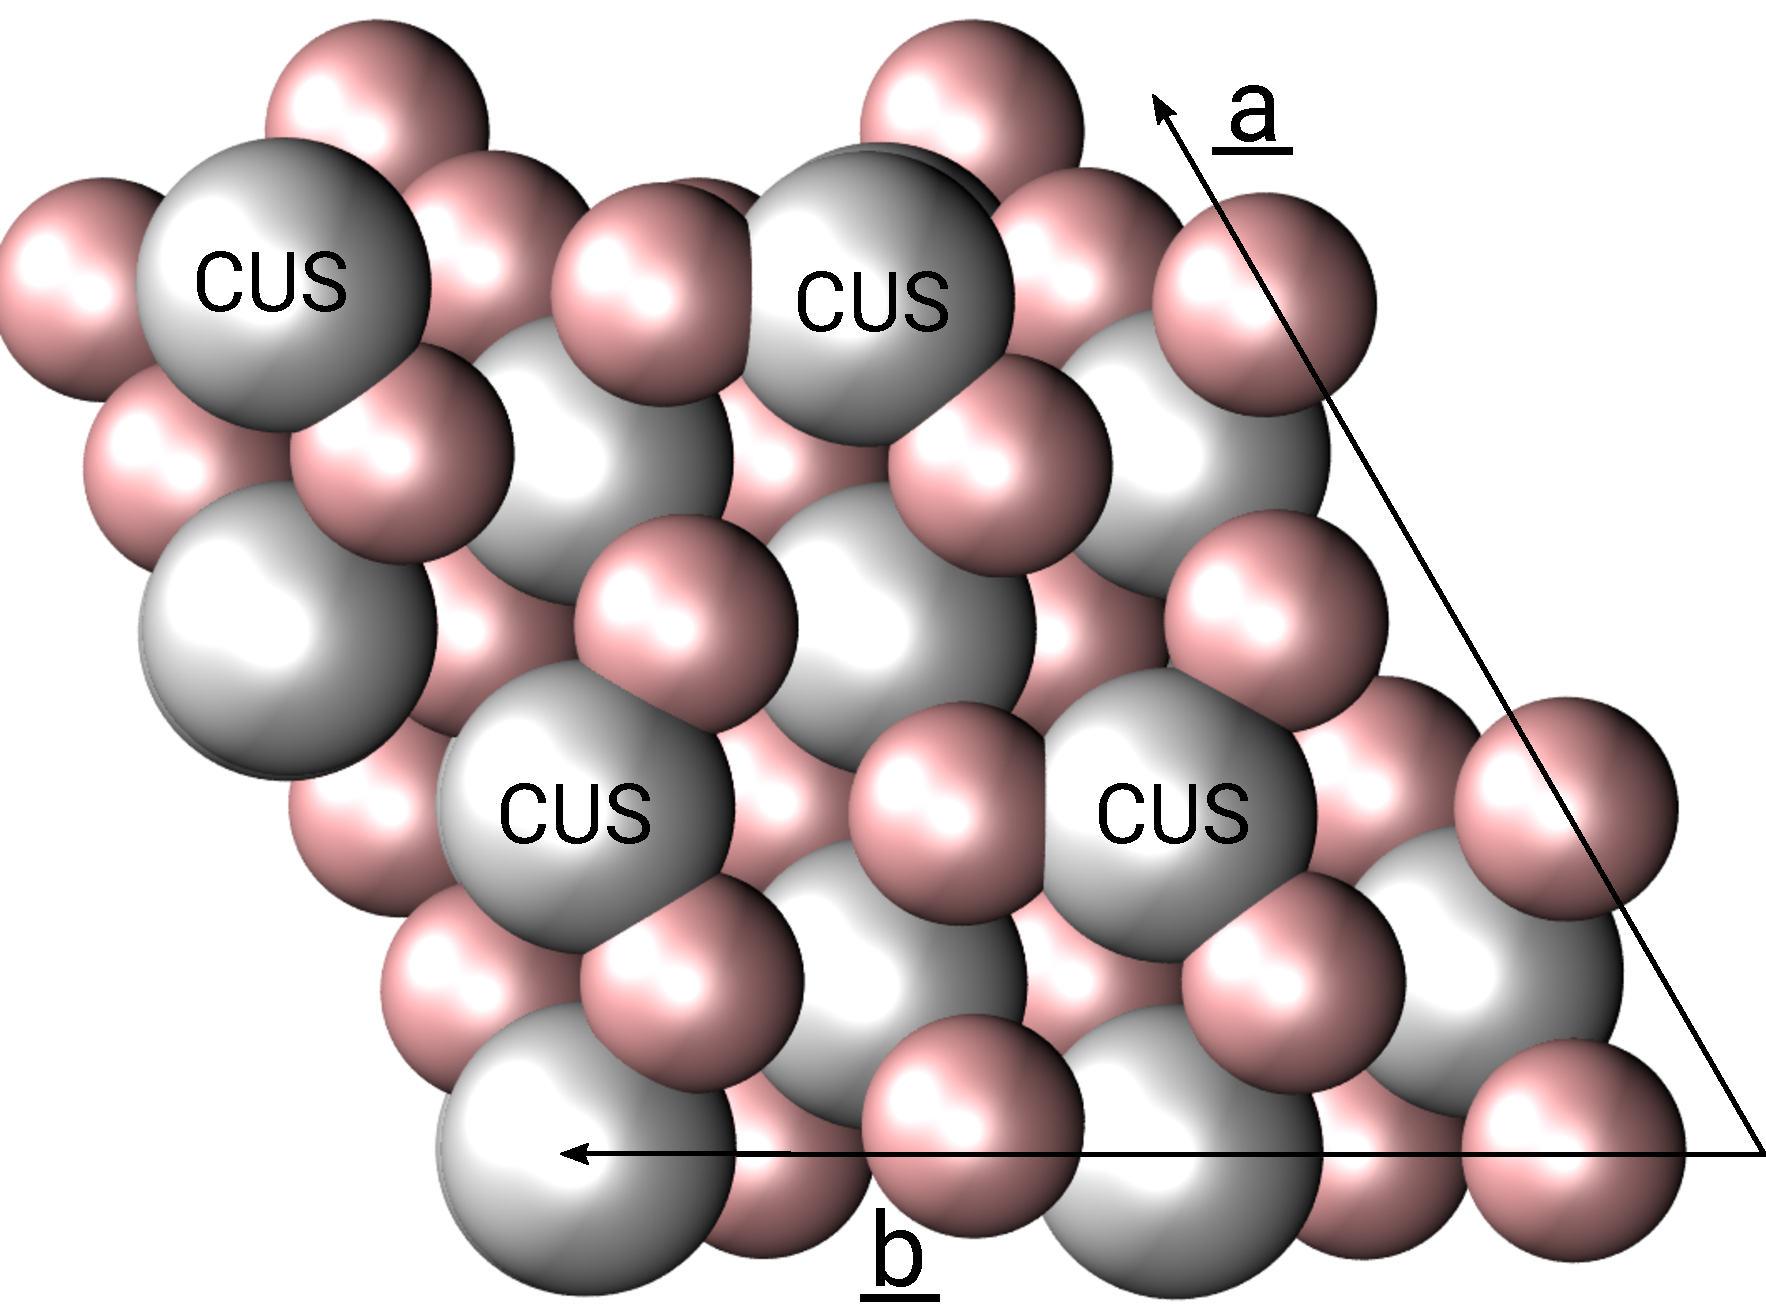
\includegraphics[width=0.45\textwidth]{figures/0001/surf_0K_axes.pdf}}
 \quad\quad
 \subfigure[(0001), side view]{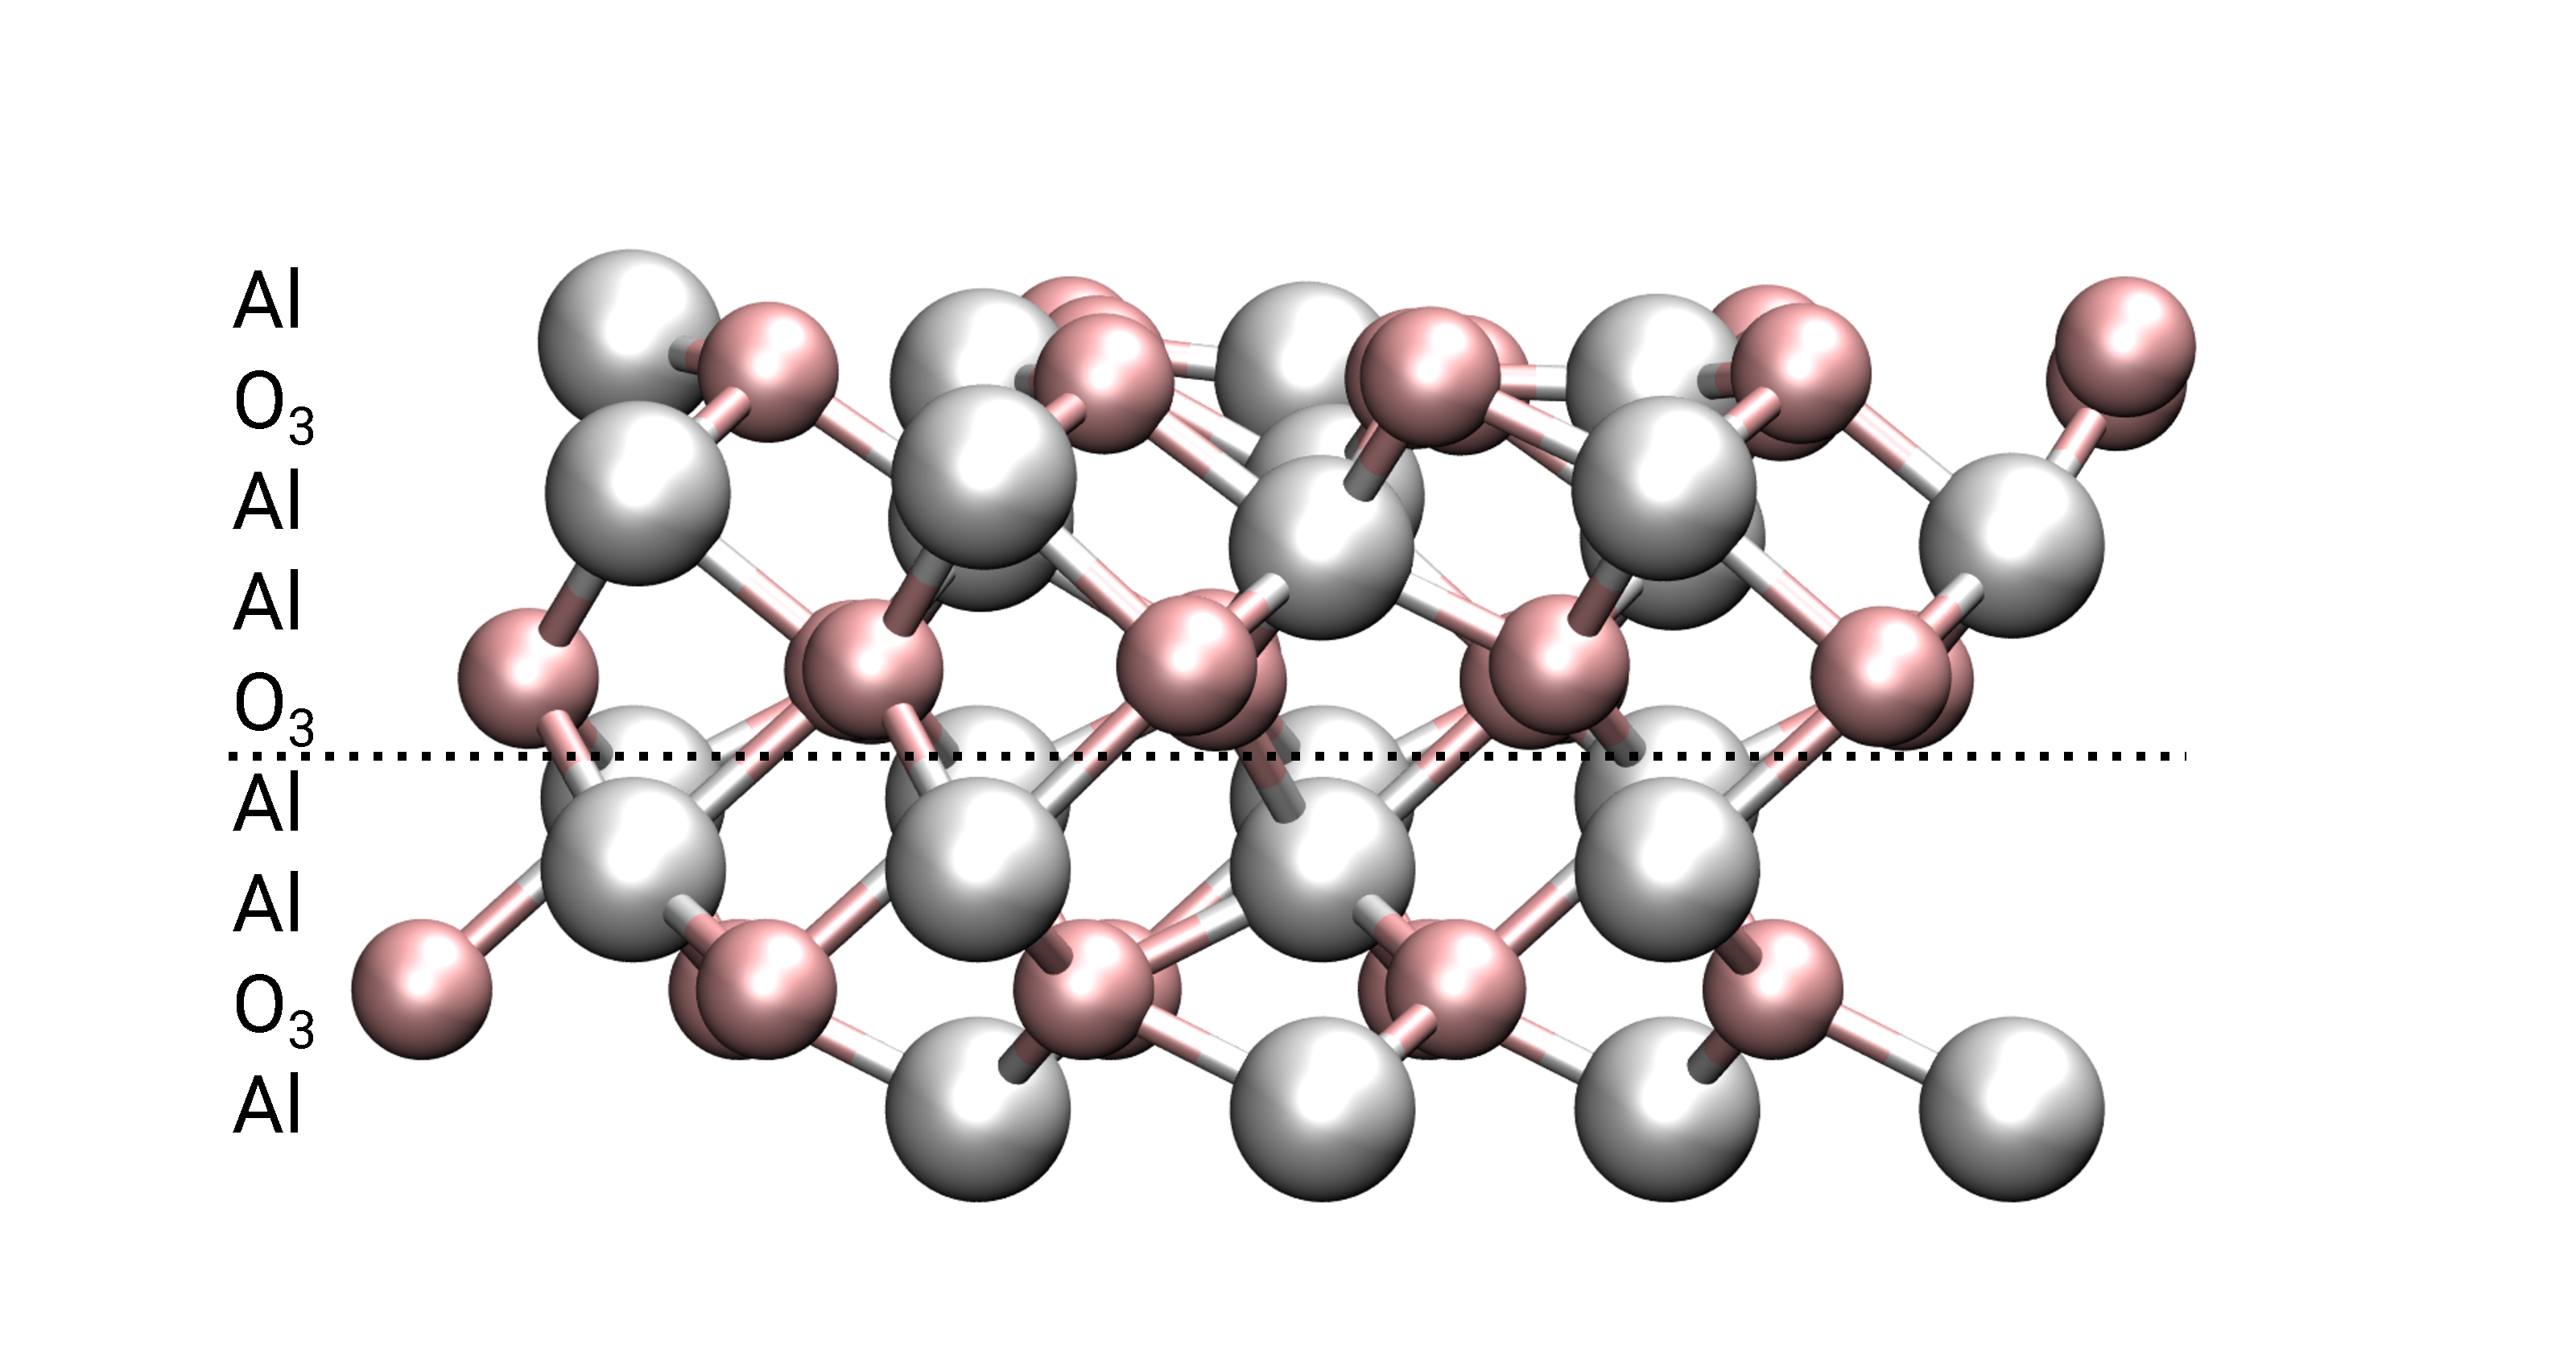
\includegraphics[width=0.45\textwidth]{figures/0001/surf_0K-side.pdf}}
 \caption{Surface model (0001).}
        \label{abb:surf_0001}
 \end{figure}

 \begin{figure*} [!ht]
\centering
\subfigure[mol]{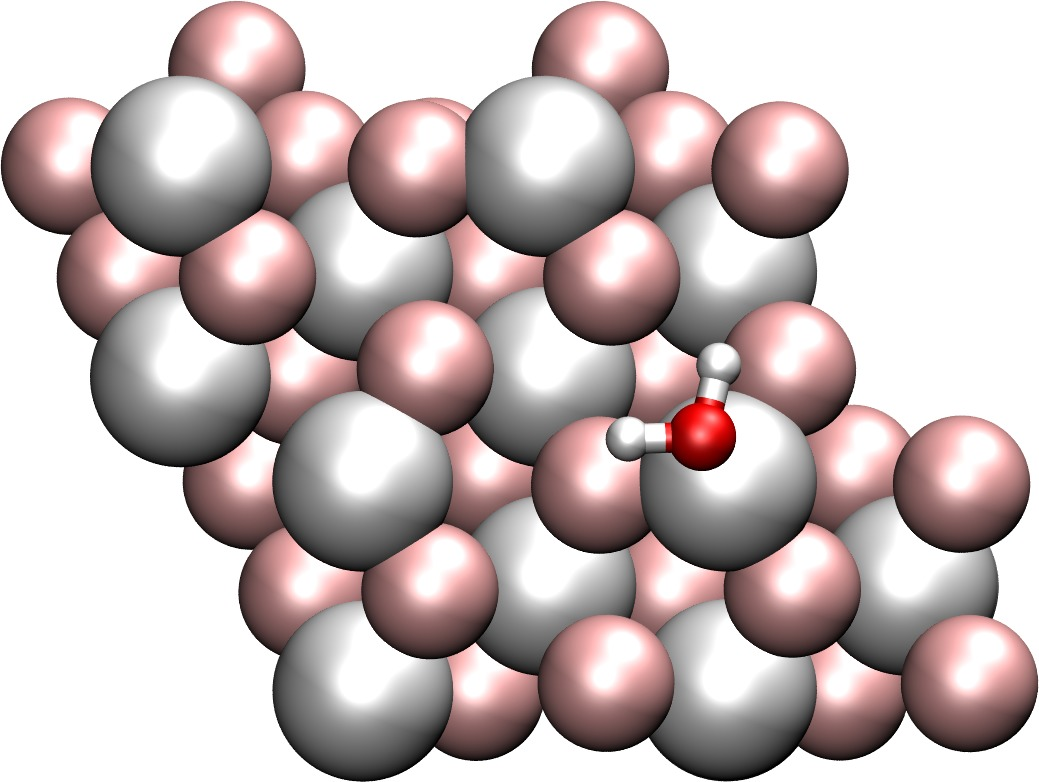
\includegraphics[width=0.4\textwidth]{figures/0001/0001_mol_top.jpg}}
         \quad
\subfigure[1-2]{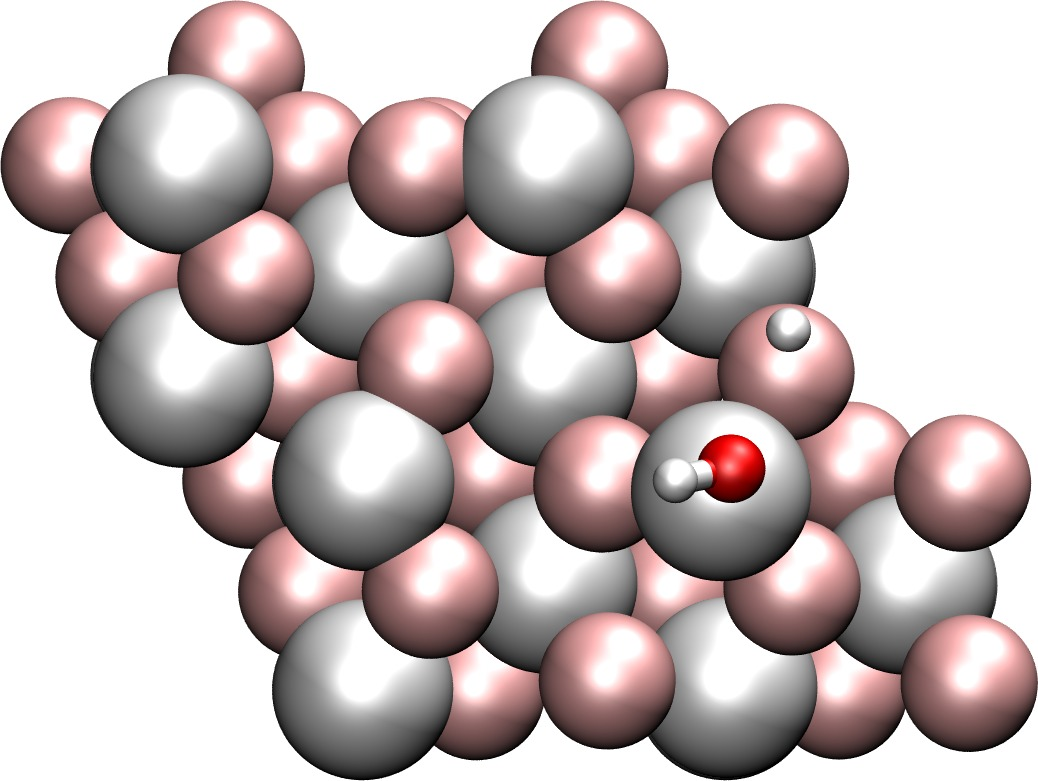
\includegraphics[width=.4\textwidth]{figures/0001/0001_1-2-diss_top.jpg}}
 \quad
\subfigure[1-4]{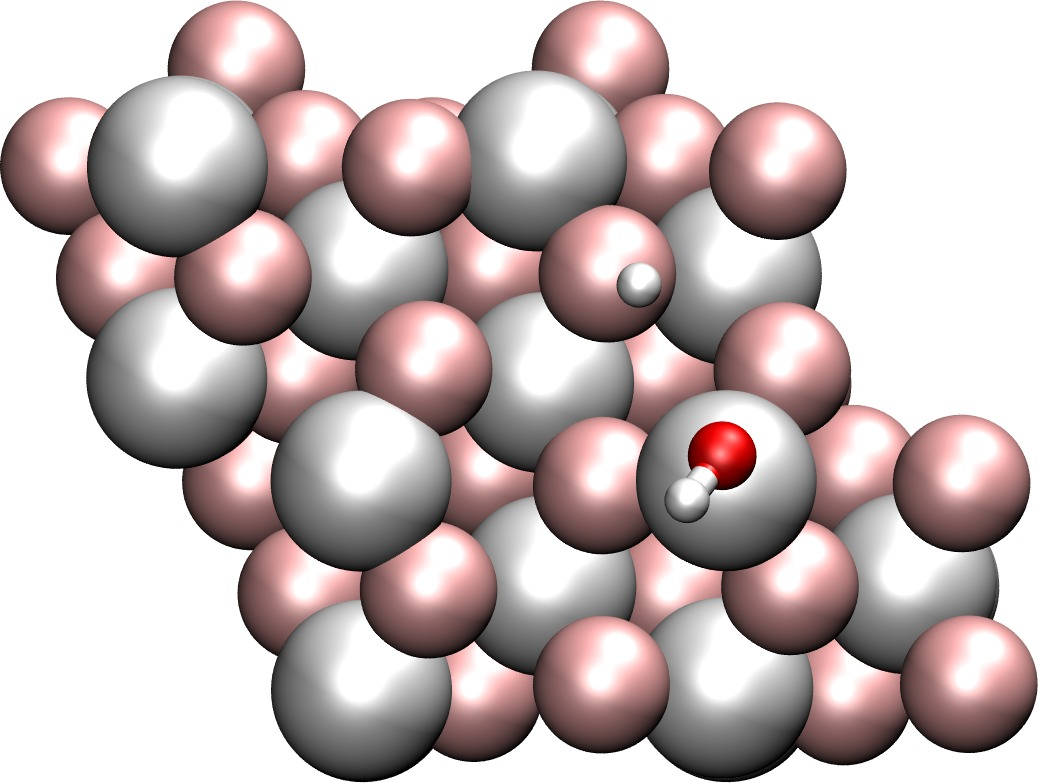
\includegraphics[width=.4\textwidth]{figures/0001/0001_1-4-diss_top.jpg}}
 \quad
\subfigure[1-4$^\prime$]{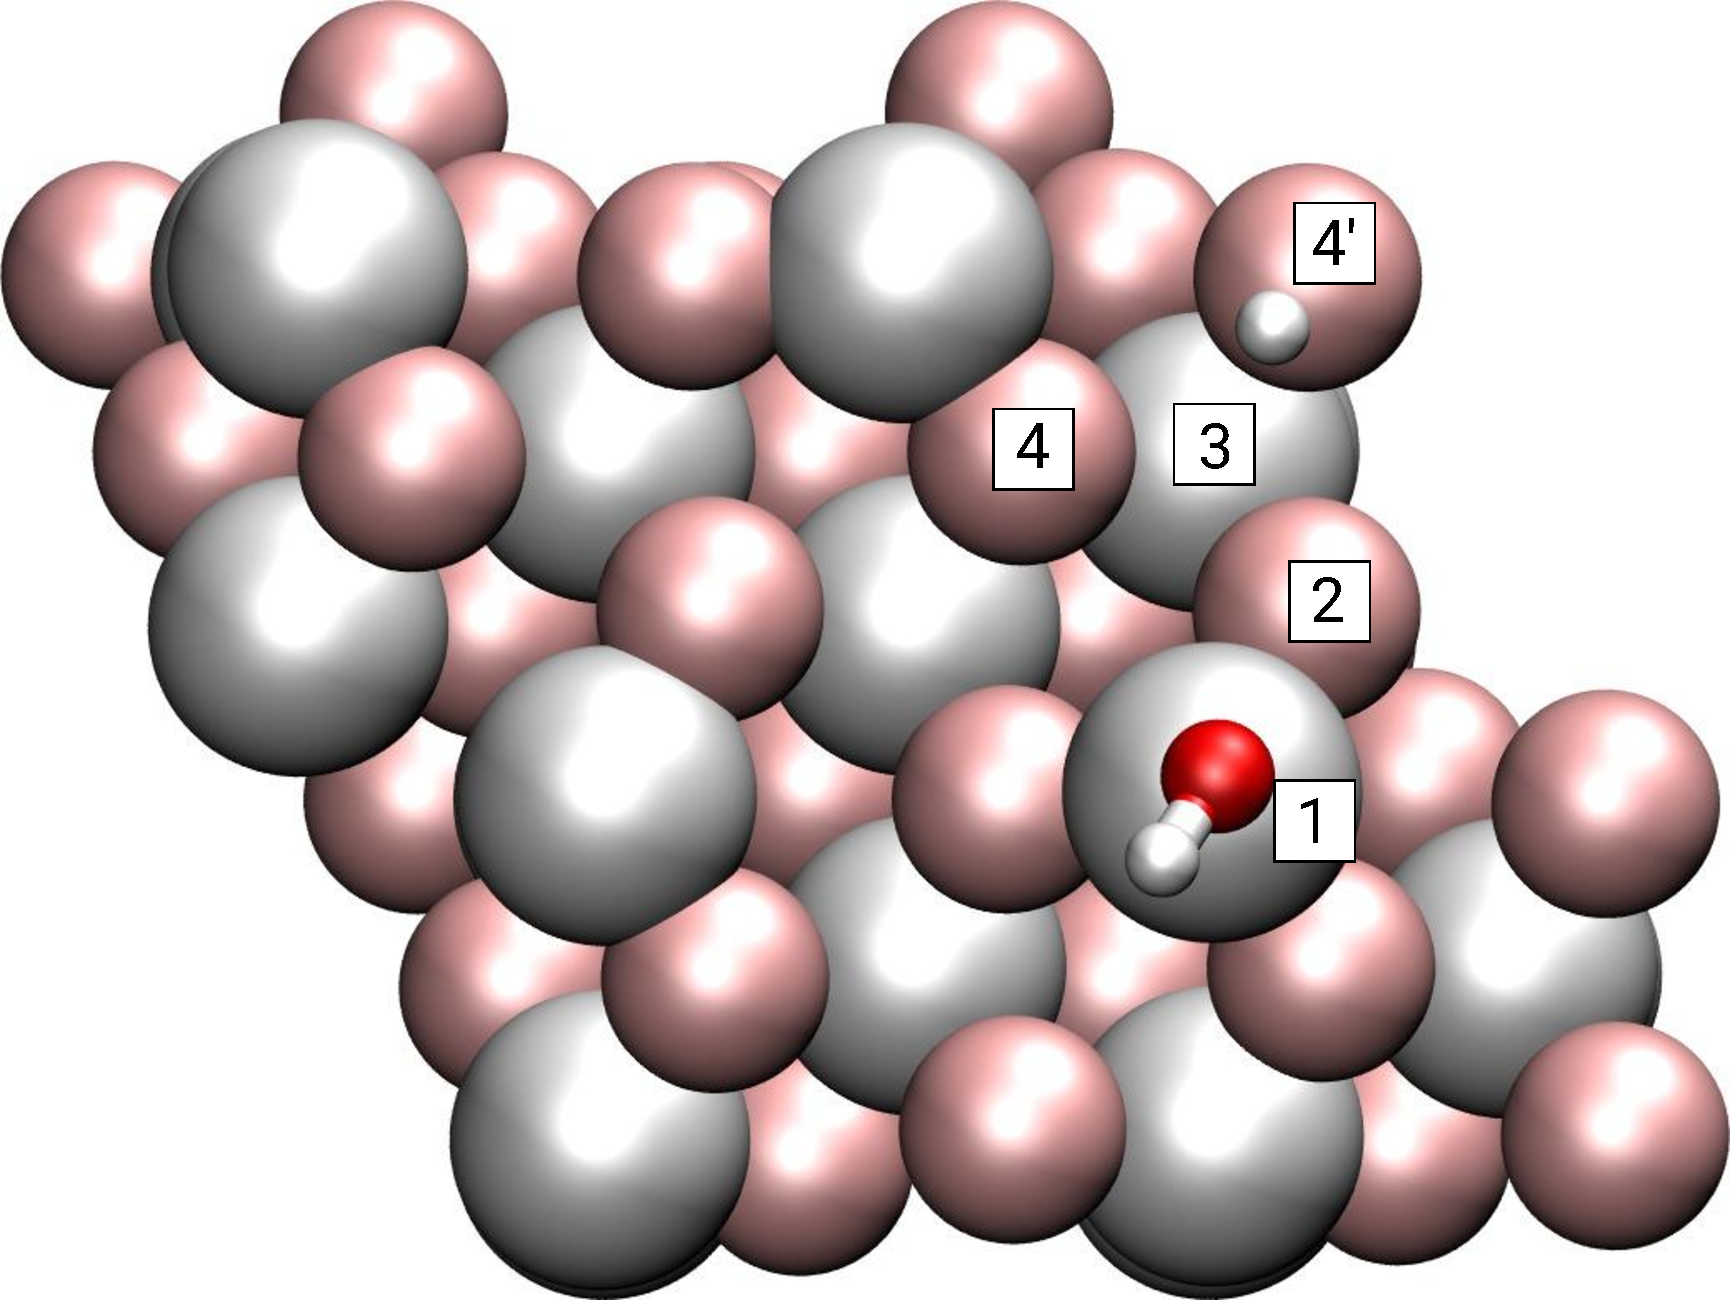
\includegraphics[width=.4\textwidth]{figures/0001/0001_1-4p-diss_top_label.pdf}}
\caption{Adsorption geometries molecular and 3 dissociated species.}
       \label{abb:0001_ads}
\end{figure*}
\section{AIMD for Dissociation Process}
Hass et. al. discussed the idea whether water will adsorb molecularly first and then dissociate or if direct dissociation upon adsorption is possible. To tackle this question for the experimental technique of the molecular beam source, we apply both microcanonical and canonical {\it ab-initio} MD to simulate the water molecules in the beam approaching the surface. We start in the low coverage limit by letting one single, rigid molecule approach the $2\times 2$ supercell. We later on continue with different approaches to more realistic beams and to more realistic surface situations. In the beam regime we probe water clusters, namely pre-optimized (H$_2$O)$_2$ and (H$_2$O)$_4$ cluster, which are shot onto the surface. Another improvement to the beam lies in having the molecule either vibrationally and/or rotationally excited. These excitations were chosen from a normal mode analysis and the resulting stretch and bending modes.
\\
For improving the surface we first use a preequilibrated surface at $300\,$K, but also go to a surface situation in which already one water molecule is adsorbed. To pay attention to the equilibrium situation we considered a molecular preadsorbed water molecule,  the most stable 1-2 dissociated state as well as the 1-4 dissociated structure.
\\
We could show that water can both dissociate upon direct contact with the surface and also dissocioate after being adsorbed molecularly first and then after a time have enough energy to dissociate. This is mostly to the 1-2 dissociated state but also 1-4 and more surprisingly 1-4$^\prime$. It seems that the rotation of the water molecule before hitting the surface is crucial for direct dissociation. This energy can also be delivered by the heated surface, it has more energy in form of vibration, in this case prolongation of the respective OH bond and can therefore lead to dissociation. On the other hand hitting the surface directly on top of a CUS atoms was shown to lead mainly to reflection of the molecule, because the energy of the incoming molecule could not be absorbed by the surface.
\\
Trajectories with the vibrationally excited modes led to statistically higher levels of dissociation. Also temperature effects of the thermalized trajectories (canonical MD) seem to have a positive influence on the dissociation.
\begin{figure}[!ht]
 \centering
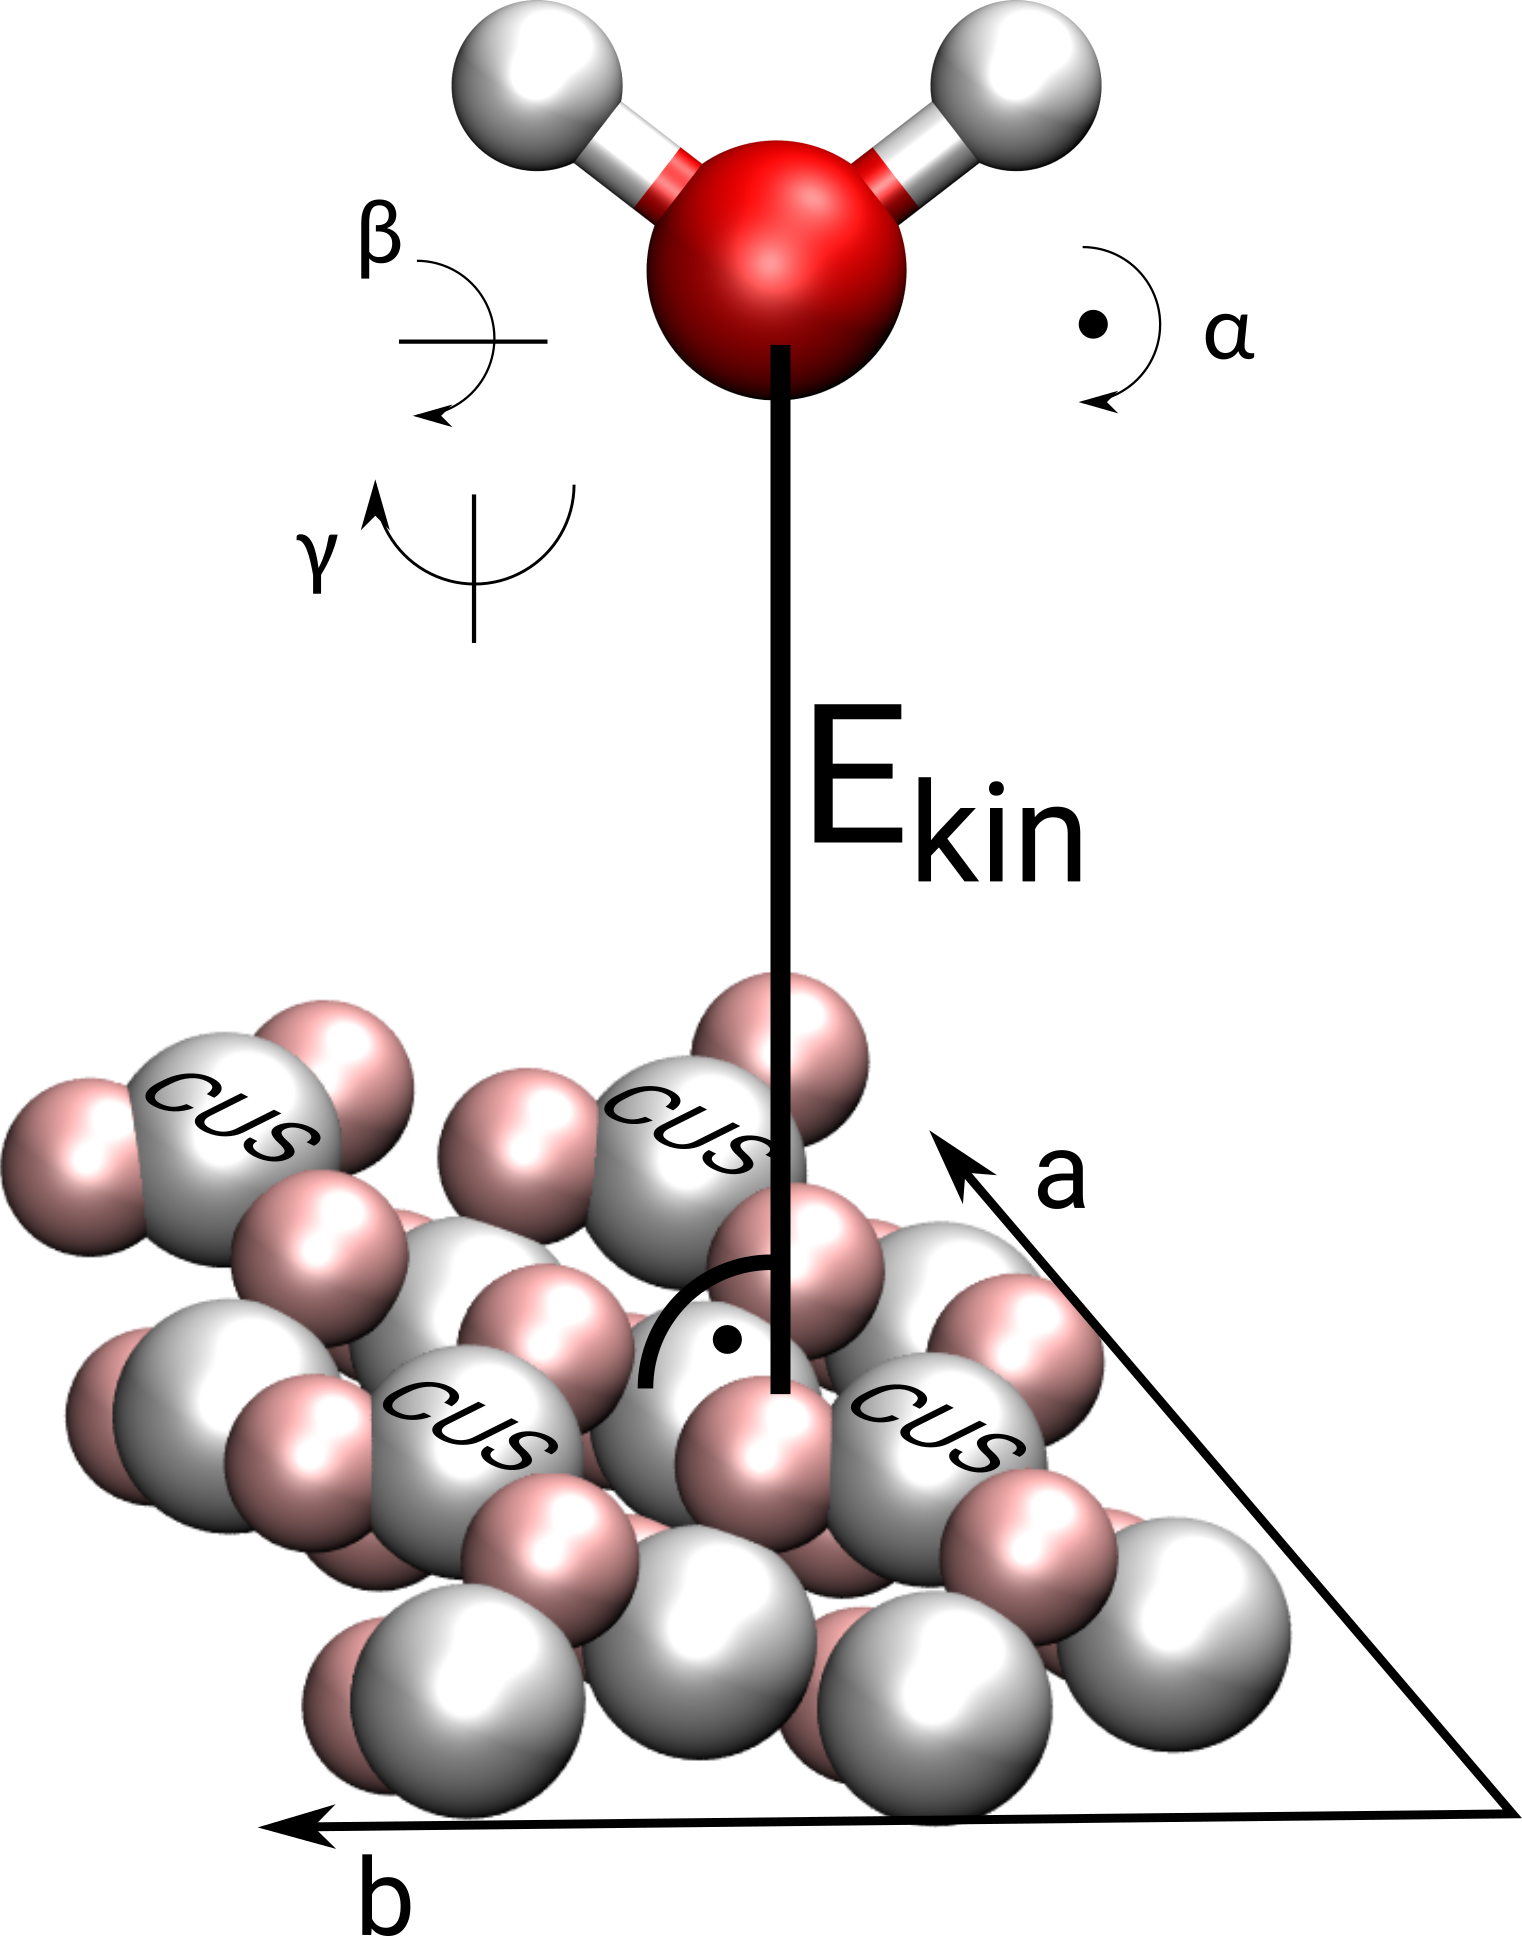
\includegraphics[width=0.4\textwidth]{figures/0001/perspective+h2o_new.png}
 \caption{Sketch for inital parameters of the trajectories.}
        \label{abb:initial_parameters}
 \end{figure}
 \subsection{Microcanonical}
\subsubsection{Cluster}
\begin{figure*} [!ht]
\centering
\subfigure[2D$_2$O]{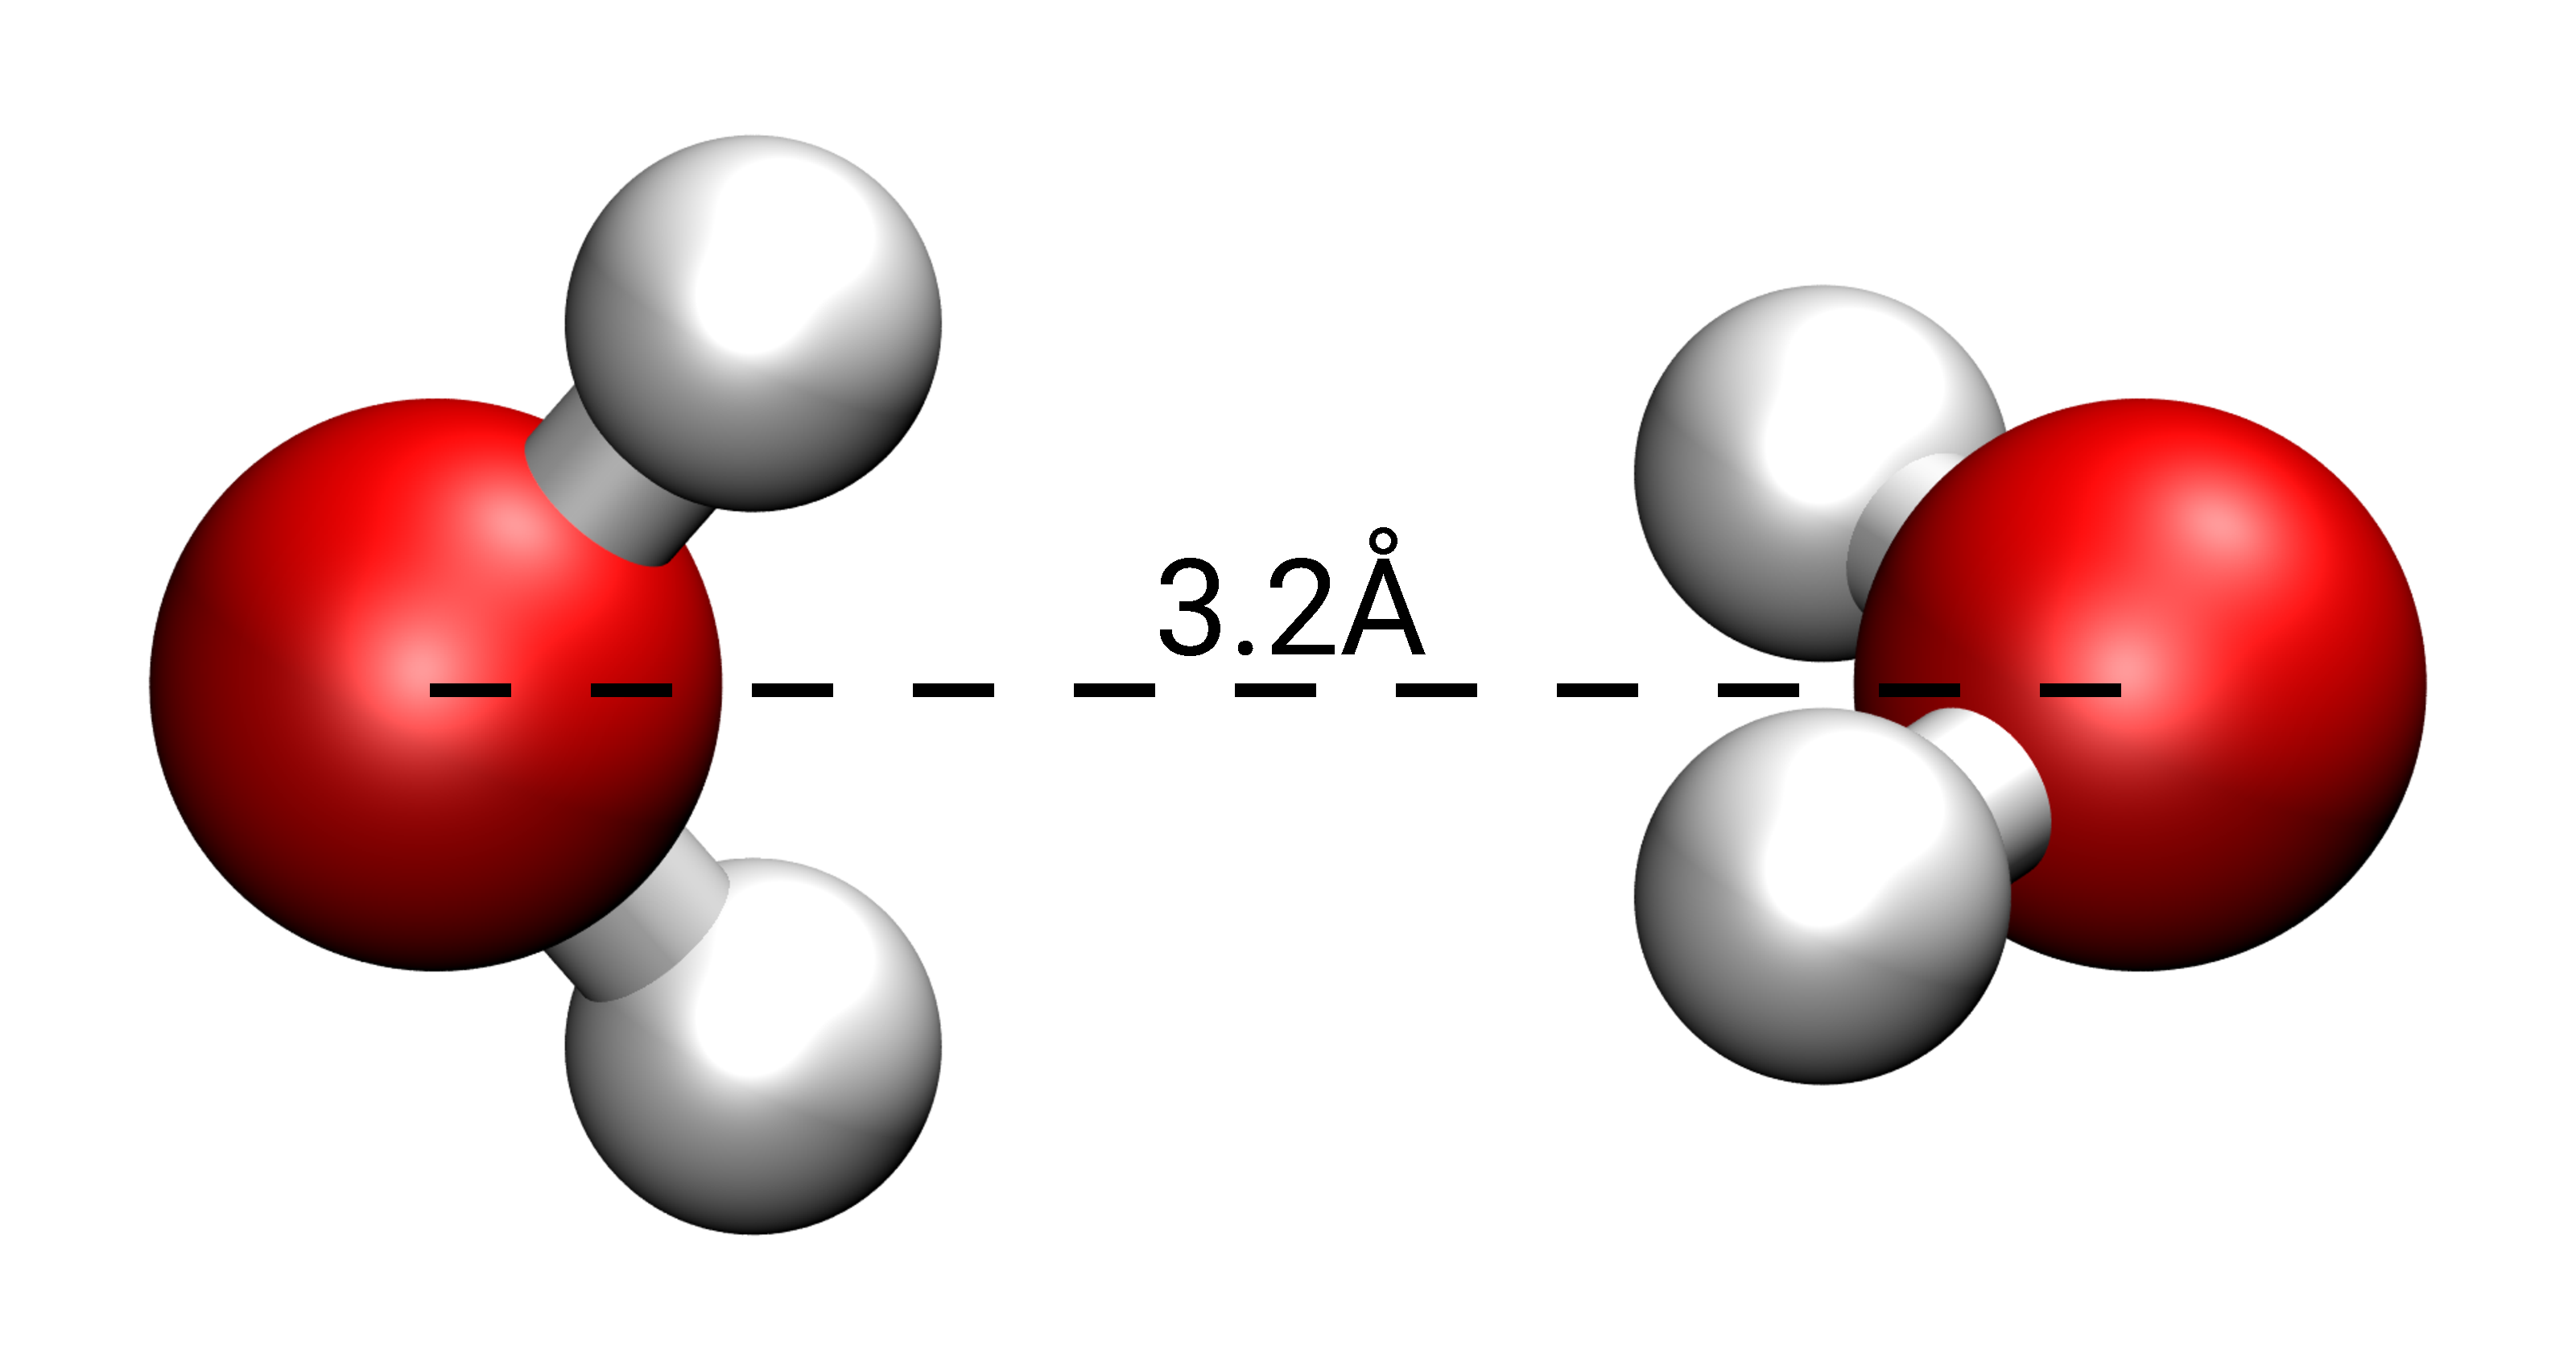
\includegraphics[width=.35\textwidth]{figures/0001/2H2O.pdf}}
 \quad
\subfigure[4D$_2$O]{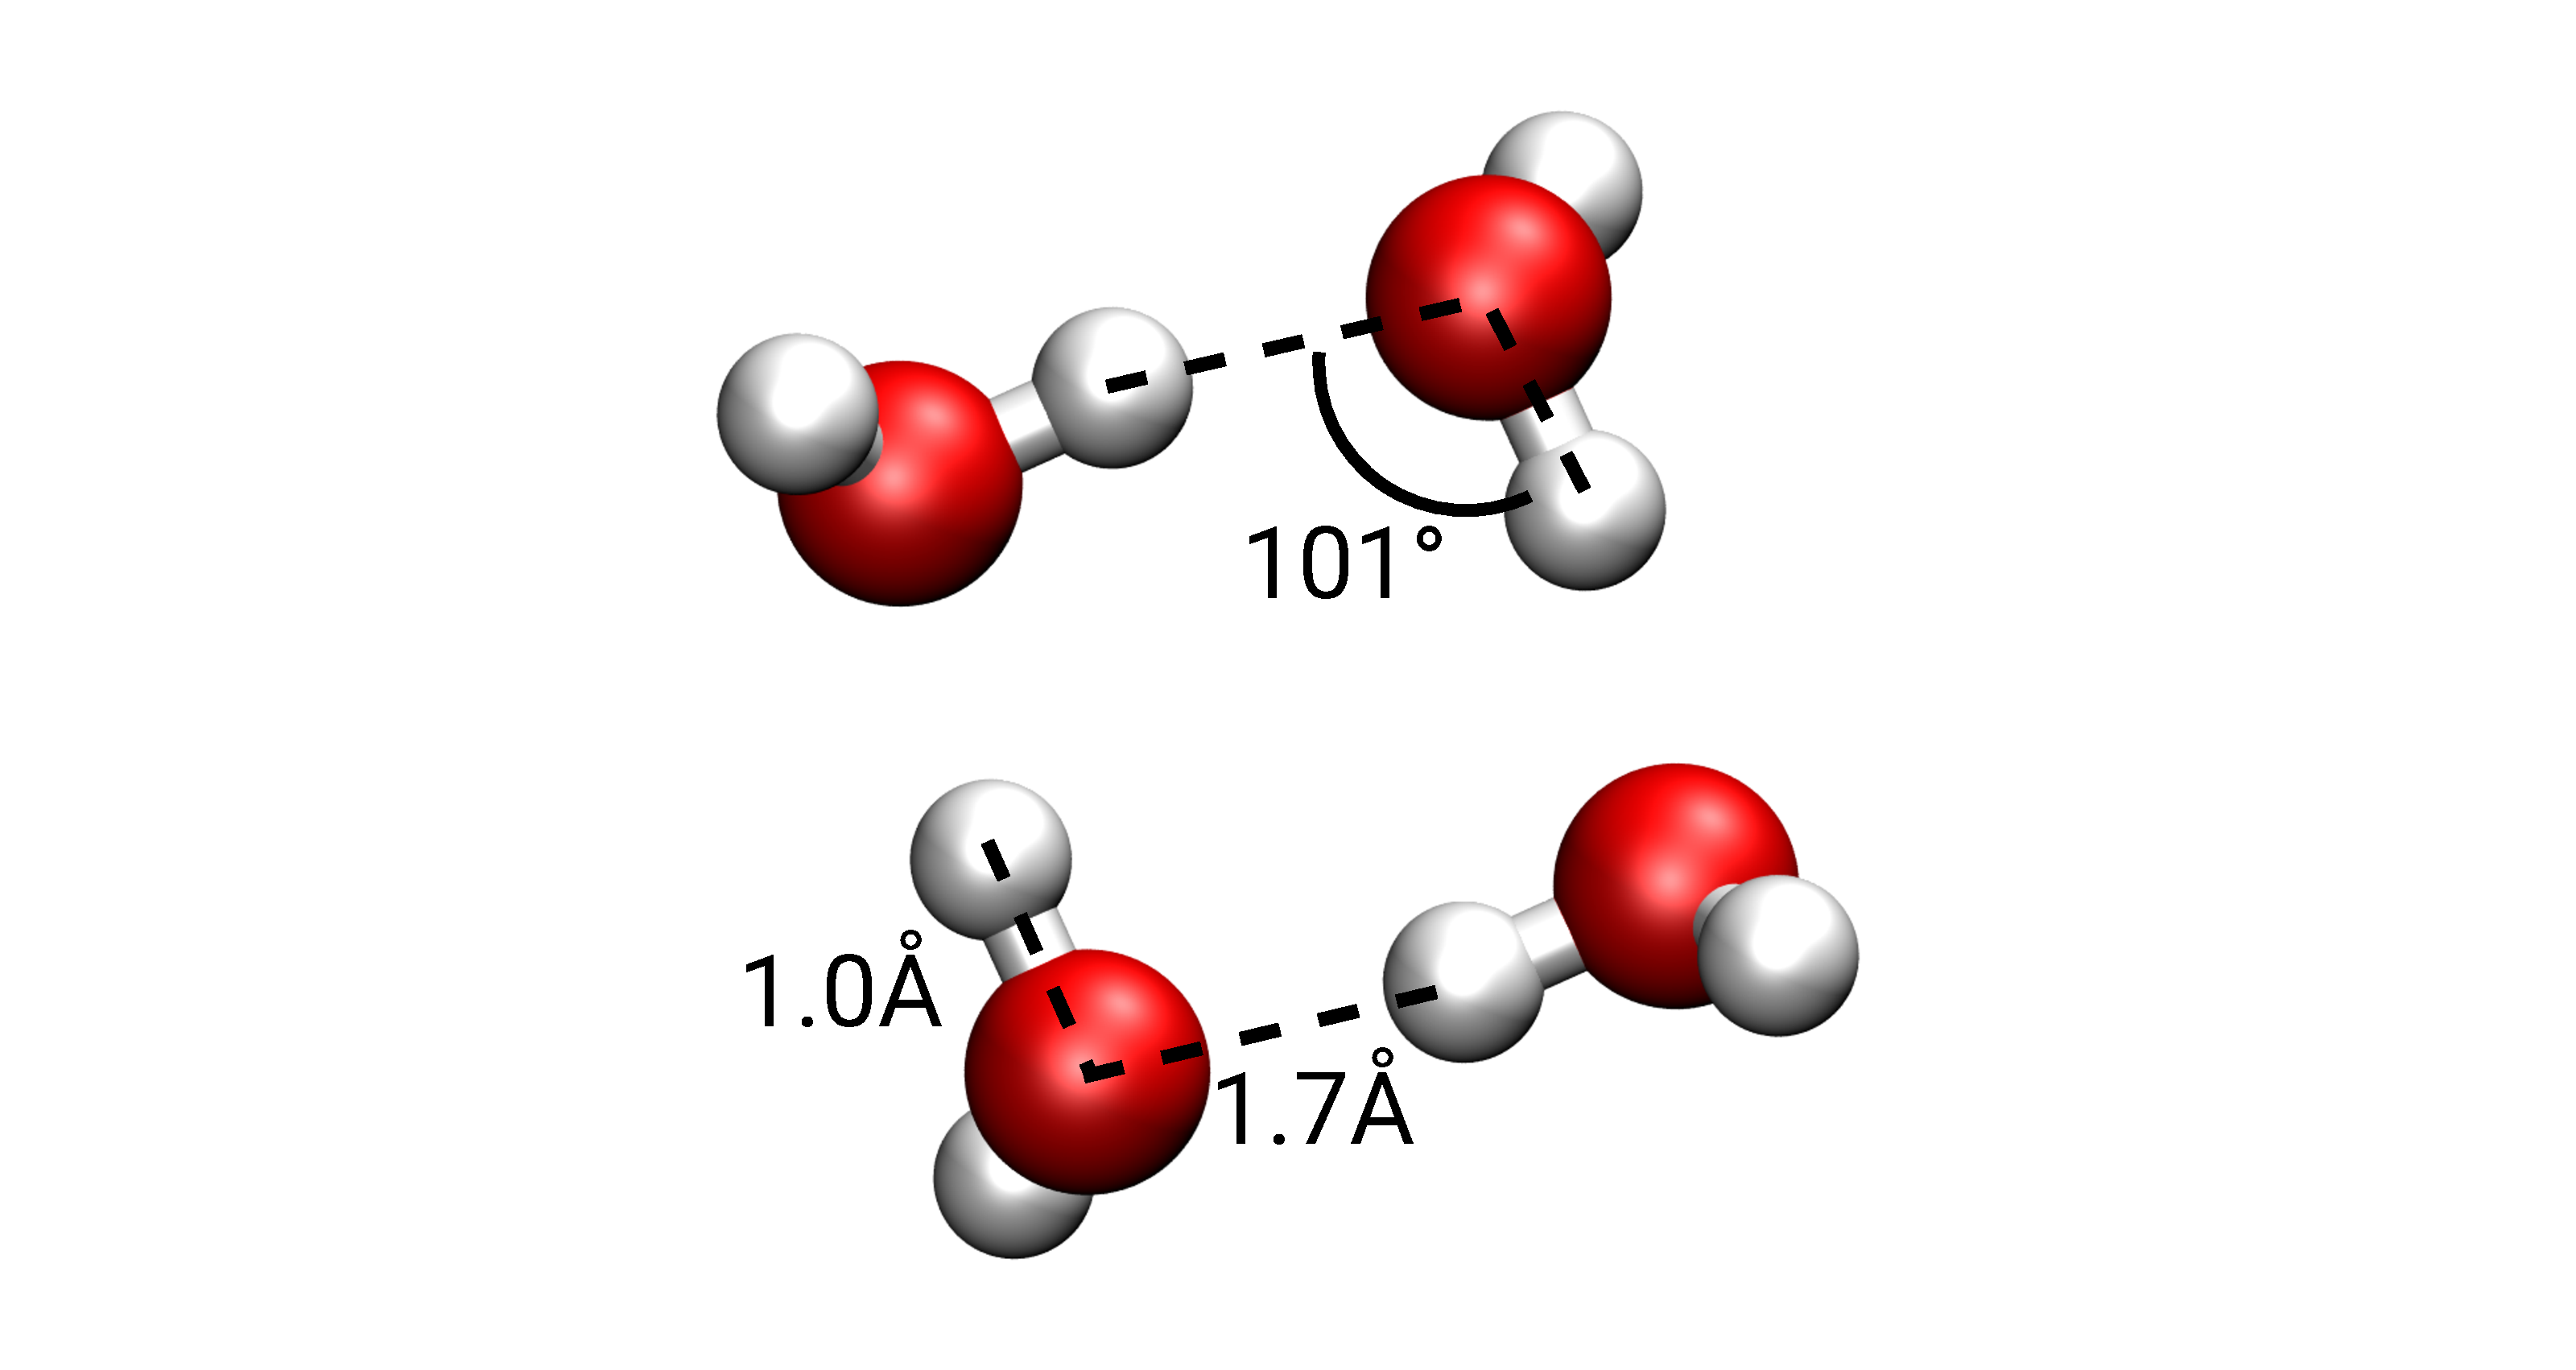
\includegraphics[width=.55\textwidth]{figures/0001/4H2O.pdf}}
\caption{Clusters for simulation of effects of higher coverages.}
       \label{abb:D2Ocluster}
\end{figure*}
\subsubsection{Preadsorbed Surface}
\subsubsection{Rotationally and Vibrationally Preexcited Water}
 \subsection{Canonical}
\clearpage
 \section{Improvement of Reaction Rates}
For a model reaction we try to improve the reaction rate with different new methods. This reaction is a H-diffusion reaction on the (0001) surface studied before in our group, the Df-H-4-2 reaction, that moves a proton in the 1-4 position to the OH residue to the 1-2 dissociated state.
The rates were before calcualted with PBE+D2/3? and Nudged Elastic Band. An approach were singlepoint calculations were done for the minima and the transition state was also done. For this process also a 1-D potential energy surface was calculated and then the Schr�dinger equation was solved to obtain the wave function and see the localization/delocalization of the reaction pathway.
\\
Now we want to expand these methods to the following 3/4/don't know? First we want to calculate the adsorption energies and the barrier within a atom centered orbital method with the hybrid functional B3LYP and also go beyond density functional theory and go to perturbation theory (LMP2).
\\
Apart from that, we study this reaction with the help of Path Integral Molecular Dynamics, where the system is represented as a couple of beads that are connected and henceforth act as a more delocalized particle which can contribute to quantum effects, proton tunneling.
\\
As a last approach, we want to apply other higher level methods in an embedded approach. We cut a cluster from the surface situation and embed this cluster in a field of point charges. By doing this we can calculate the cluster with a better method, let's say B3LYP, CCSD or MP2 and then apply a substractional scheme to get to corrected adsorption energies that can then be used to improve the rates with Eyring's equation for transtition states.

\subsection{MP2 and B3LYP}
Going beyond pure density functionals and also beyond DFT has been too costly for a long time, simply not applicable for surface adsorbat system that large and electron rich. In the crystal/cryscor code one uses atom centered bases instead of plane waves and so large scale systems can also be computed. We first optimized our parameters with HF calculations and then did calculations with PBE similar to prior plane wave based calculations.
\\
We found out, that BSSE takes a big part, but corrections are not easily applied because the ghosted calculations needed for that do not converge for all the structures with a bigger OH-H distance. Instead we have to use bigger basis sets containing diffuse functions in order to handle the BSSE. Such a self designed basis set by our cooperation partner Dr. Denis Usvyat (HU Berlin, group of Martin Sch\"utz) was used here. With this basis set we did the PBE calculations again (?) and the B3LYP as well as the MP2 calculations. First we compared the differences in adsorption energies. We furthermore compared the vibrational frequencies from B3LYP with the ones from VASP/PBE to see a methodological effect.
\\
We also reoptimized the transition state for the Df-H-4-2 reaction.



{\color{red} Not sure if this will come into the diss? No real results obtained..?}
\subsection{PIMD}
Instead of calculating rates with a defined reaction pathway, we use the path integral MD to propagate the 1-4 dissociated state in the hope to watch the reaction and calculate the rate from that. But unluckily, no reaction occurred in the given propagation time, so that one only can see the delocalization of the proton. At a given temperature of $300\,$K the proton only moves a little, far away from any reactive trajectory.
\\
 A huge problem was the unit cell: when all atoms or only a few atoms were allowed to move during the trajectory, the whole cell drifted away, as if the periodic boundary conditions would not apply. When fixing all the atoms except for the proton that diffuses it was fine.
 \\
 {\color{red} cell optimizations were tried, but didn't work as planned; fixing only the rim lead to other atom's movement, maybe one can free the OH group and the Al atom on which the H sits?}
 \\
 We used also PBE but without dispersion corrections and for the trajectories at $300\,$K we applied the Nos\'{e} Hoover thermostat.
 
\subsection{QM/QM Embedding Scheme}
In order to recalculate adsorption energies and reaction rate constants with a higher level method we try to apply the mechanical embedding scheme developed in the Sauer group from HU Berlin. One uses a substractive scheme to correct energies, after calculating the complete system with the low level method (here PBE), the interesting part, namely the cluster, with both the low level method and the high level method (B3LYP, MP2 or CCSD). The high-level:low-level corrected energy is then calculated by the following equation: {\it equation}
\\
First of all, a reasonable cluster has to be chosen, which is difficult since the 1-4$^\prime$ needs a big cluster to be considered. We chose then the Al$_8$O$_{12}$-cluster used in unpublished work from the same group. This cluster was used for tests but when it came to embedding, the Turbomole package failed to compute the embedded system, because hexagonal cells were not yet implemented into the code.


\addchap{Summary}

We made great progress in understanding the (11\=20) surface of $\upalpha$-Al$_2$O$_3$ in contact with water in the low coverage regime. 
\\
The dissociation process of water on (0001) surface was studied.
\\
Several methods were tested to improve reaction rates.
%%%%%%%%%%%%%%%%%%%%%%%%%%%%%%%%%%%%%%%%%%%%%%%%%%%%%%%%%%%%%%%%%%%%%%%%%%%%%%%%%%%%%%%%%%%%%%%%%%%%%%%%%%%%%%%%%%%%%%%%%%%%%%%%%%%%%%%%%%%%%%%%%%%%%%%%%%%%%%%%%%%%%%%%%%%%%%%%%%%%%%%%%%%%%%%%%%%%%%%%%%%%%%%%%%%%%%%%%%%%%%%%%%%%%%%%%%%%%%%%%%%%%%%%%%%%%%%%%%%%%%%

\begingroup
\renewcommand{\cleardoublepage}{}
\clearpage
\addchap*{Acknowledgment}
\endgroup
I want to thank my doctoral father Prof. Dr. Saalfrank, for giving me the scientific opportunity to research on surface systems and all the valuable discussions and advices. my first supervisor Dr. Jonas Wirth who gave me support during my time starting as a Bachelor's student, during my Master's thesis and also through the beginning of my PhD, PD Dr. Tillmann Klamroth for discussions about programming and theoretical questions that arose during the work, Dr. Rados\l{}aw W\l{}odarczyk for his endless knowledge with vasp and programming in general, Giacomo Melani (soon to be Dr.) for his advice and his help, and also the discussions about our teaching duties in mathematics and the whole workgroup for all the valuable discussions and the help. Also for the great atmosphere, that was some times productive and some times also just relaxing and felt very comfortable, here especially Clemens Rietze, Robert Scholz, Gereon Floss, and Steven Lindner.
Also I want to thank my cooperation partners from FHI, Yanhua Yue, Dr. Harald Kirsch and Dr. Kramer R. Campen for the great work and publications we did together.
Thanks to Dr. Denis Usvyat for all his patience and knowledge and valuable discussions about crystal/cryscor and his help.

%%%%%%%%%%%%%%%%%%%%%%%%%%%%%%%%%%%%%%%%%%%%%%%%%%%%%%%%%%%%%%%%%%%%%%%%%%%%%%%%%%%%%%%%%%%%%%%%%%%%%%%%%%%%%%%%%%%%%%%%%%%%%%%%%%%%%%%%%%%%%%%%%%%%%%%%%%%%%%%%%%%%%%%%%%%%%%%%%%%%%%%%%%%%%%%%%%%%%%%%%%%%%%%%%%%%%%%%%%%%%%%%%%%%%%%%%%%%%%%%%%%%%%%%%%%%%%%%%%%%%%%
%%%%%%%%%%%%%%%%%%%%%%%%%%%%%%%%%%%%%%%%%%%%%%%%%%%%%%%%%%%%%%%%%%%%%%%%%%%%%%%%%%%%%%%%%%%%%%%%%%%%%%%%%%%%%%%%%%%%%%%%%%%%%%%%%%%%%%%%%%%%%%%%%%%%%%%%%%%%%%%%%%%%%%%%%%%%%%%%%%%%%%%%%%%%%%%%%%%%%%%%%%%%%%%%%%%%%%%%%%%%%%%%%%%%%%%%%%%%%%%%%%%%%%%%%%%%%%%%%%%%%%%
%%%%%%%%%%%%%%%%%%%%%%%%%%%%%%%%%%%%%%%%%%%%%%%%%%%%%%%%%%%%%%%%%%%%%%%%%%%%%%%%%%%%%%%%%%%%%%%%%%%%%%%%%%%%%%%%%%%%%%%%%%%%%%%%%%%%%%%%%%%%%%%%%%%%%%%%%%%%%%%%%%%%%%%%%%%%%%%%%%%%%%%%%%%%%%%%%%%%%%%%%%%%%%%%%%%%%%%%%%%%%%%%%%%%%%%%%%%%%%%%%%%%%%%%%%%%%%%%%%%%%%%

\appendix

%\begingroup
%\renewcommand{\cleardoublepage}{}
%\renewcommand{\clearpage}{}
%\clearpage
%\renewcommand*{\chapterheadstartvskip}{\vspace*{-\baselineskip}}
\addchap{Appendix}
%\endgroup


%%%%%%%%%%%%%%%%%%%%%%%%%%%%%%%%%%%%%%%%%%%%%%%%%%%%%%%%%%%%%%%%%%%%%%%%%%%%%%%%%%%%%%%%%%%%%%%%%%%%%%%%%%%%%%%%%%%%%%%%%%%%%%%%%%%%%%%%%%%%%%%%%%%%%%%%%%%%%%%%%%%%%%%%%%%%%%%%%%%%%%%%%%%%%%%%%%%%%%%%%%%%%%%%%%%%%%%%%%%%%%%%%%%%%%%%%%%%%%%%%%%%%%%%%%%%%%%%%%%%%%%
%%%%%%%%%%%%%%%%%%%%%%%%%%%%%%%%%%%%%%%%%%%%%%%%%%%%%%%%%%%%%%%%%%%%%%%%%%%%%%%%%%%%%%%%%%%%%%%%%%%%%%%%%%%%%%%%%%%%%%%%%%%%%%%%%%%%%%%%%%%%%%%%%%%%%%%%%%%%%%%%%%%%%%%%%%%%%%%%%%%%%%%%%%%%%%%%%%%%%%%%%%%%%%%%%%%%%%%%%%%%%%%%%%%%%%%%%%%%%%%%%%%%%%%%%%%%%%%%%%%%%%%
%%%%%%%%%%%%%%%%%%%%%%%%%%%%%%%%%%%%%%%%%%%%%%%%%%%%%%%%%%%%%%%%%%%%%%%%%%%%%%%%%%%%%%%%%%%%%%%%%%%%%%%%%%%%%%%%%%%%%%%%%%%%%%%%%%%%%%%%%%%%%%%%%%%%%%%%%%%%%%%%%%%%%%%%%%%%%%%%%%%%%%%%%%%%%%%%%%%%%%%%%%%%%%%%%%%%%%%%%%%%%%%%%%%%%%%%%%%%%%%%%%%%%%%%%%%%%%%%%%%%%%%

\begingroup
\renewcommand{\cleardoublepage}{}
~
\clearpage
~
\clearpage
\addchap*{Publications}
\endgroup

\subsubsection{This Work:}

\begin{enumerate}[itemsep=0.25\baselineskip]
%  \item \bibentry{Wirth12}.
  \item Heiden, S.; Yue, Y.; Kirsch, H.; Wirth, J.; Saalfrank, P.; Campen, R. K.: {\frqq}title{\flqq}, {\it Journal} {\bf year,} {\it vol,} pp.
  \item Heiden, S.;  Saalfrank, P.: {\frqq}title{\flqq}, {\it Journal} {\bf year,} {\it vol,} pp.

\end{enumerate}



%%%%%%%%%%%%%%%%%%%%%%%%%%%%%%%%%%%%%%%%%%%%%%%%%%%%%%%%%%%%%%%%%%%%%%%%%%%%%%%%%%%%%%%%%%%%%%%%%%%%%%%%%%%%%%%%%%%%%%%%%%%%%%%%%%%%%%%%%%%%%%%%%%%%%%%%%%%%%%%%%%%%%%%%%%%%%%%%%%%%%%%%%%%%%%%%%%%%%%%%%%%%%%%%%%%%%%%%%%%%%%%%%%%%%%%%%%%%%%%%%%%%%%%%%%%%%%%%%%%%%%%

\addchap{References}
\begingroup
\let\clearpage\relax
\renewcommand*{\chapterheadstartvskip}{\vspace*{-2\baselineskip}}
\begin{small}
\bibliographystyle{achemso_mod}
%\addcontentsline{toc}{chapter}{Literaturverzeichnis}
%\bibliography{literatur}
\end{small}
\endgroup

%\renewcommand*\listfigurename{Bildverzeichnis}
%\makeatletter\renewcommand\numberline[1]{}\listoffigures
%\addcontentsline{toc}{paragraph}{Bildverzeichnis}

%%%%%%%%%%%%%%%%%%%%%%%%%%%%%%%%%%%%%%%%%%%%%%%%%%%%%%%%%%%%%%%%%%%%%%%%%%%%%%%%%%%%%%%%%%%%%%%%%%%%%%%%%%%%%%%%%%%%%%%%%%%%%%%%%%%%%%%%%%%%%%%%%%%%%%%%%%%%%%%%%%%%%%%%%%%%%%%%%%%%%%%%%%%%%%%%%%%%%%%%%%%%%%%%%%%%%%%%%%%%%%%%%%%%%%%%%%%%%%%%%%%%%%%%%%%%%%%%%%%%%%%

\clearpage

\begin{center}
  {\Large\sffamily\bfseries Erkl�rung}
\end{center}

\vspace{\baselineskip}

Hiermit versichere ich, dass die vorliegende Arbeit an keiner anderen Hochschule eingereicht sowie selbst�ndig und ausschlie�lich mit den angegebenen Mitteln angefertigt worden ist.\\

\begin{flushleft}
  Potsdam, xx 2018
\end{flushleft}

\end{document}
